\documentclass[a4paper,twoside]{article}
\usepackage{microtype}

\usepackage{epsfig}
\usepackage{subcaption}
\usepackage{calc}
\usepackage{amssymb}
\usepackage{amstext}
\usepackage{amsmath}
\usepackage{amsthm}
\usepackage{multicol}
\usepackage{pslatex}
\usepackage{apalike}

\usepackage{csquotes}
\usepackage[hidelinks]{hyperref}
\usepackage{algorithm2e}
\usepackage[table,dvipsnames,cmyk]{xcolor}
\usepackage{tabularx}
\usepackage{booktabs}

\usepackage{pifont}
\newcommand*\OK{$\circ$}
\newcommand*\OKbf{$\bullet$}

\newcommand*\rot{\rotatebox{90}}

\newcommand*\Ts {$\mathcal{T}_{\mathrm{S}}$}
\newcommand*\Tc {$\mathcal{T}_{\mathrm{C}}$}
\newcommand*\Tie{$\mathcal{T}_{\mathrm{IE}}$}
\newcommand*\Tmt{$\mathcal{T}_{\mathrm{MT}}$}
\newcommand*\Th{$\mathcal{H}$}

\definecolor{darkred}{RGB}{177,  6, 58}
\newcommand*\redify{\textcolor{darkred}}

\usepackage{tikz}
\usetikzlibrary{trees,calc,fit,backgrounds,positioning,shapes,arrows.meta,spy,3d,calendar,shapes.multipart}

\makeatletter
\tikzset{inside/.code=\preto\tikz@auto@anchor{\pgf@x-\pgf@x\pgf@y-\pgf@y}}
\makeatother

\usepackage{tikz-pipeline}

\usepackage{wrapfig}
\usepackage{tabularx}

\usepackage{placeins}

\usepackage{afterpage}

\tikzset{
	-|-/.style={
		to path={
			(\tikztostart) -| ($(\tikztostart)!#1!(\tikztotarget)$) |- (\tikztotarget)
			\tikztonodes
		}
	},
	-|-/.default=0.5,
	|-|/.style={
		to path={
			(\tikztostart) |- ($(\tikztostart)!#1!(\tikztotarget)$) -| (\tikztotarget)
			\tikztonodes
		}
	},
	|-|/.default=0.5,
}

\usepackage{SCITEPRESS}     %

\begin{document}

\title{A Taxonomy of Treemap Visualization Techniques}

\author{%
	\authorname{%
		Willy Scheibel~\orcidAuthor{0000-0002-7885-9857}%
		, Matthias Trapp~\orcidAuthor{0000-0003-3861-5759}%
		, Daniel Limberger~\orcidAuthor{0000-0002-9111-4809}%
		~and J{\"u}rgen D{\"o}llner}%
	\affiliation{Hasso Plattner Institute, Faculty of Digital Engineering, University of Potsdam, %
		Germany}
}

\abstract{%
	A treemap is a visualization that has been specifically designed to facilitate the exploration of tree-structured data and, more general, hierarchically structured data.
	The family of visualization techniques that use a visual metaphor for parent-child relationships based \enquote{on the property of containment}~\cite{johnson1993-categorical} is commonly referred to as treemaps.
	However, as the number of variations of treemaps grows, it becomes increasingly important to distinguish clearly between techniques and their specific characteristics.
	This paper proposes to discern between \emph{Space-filling Treemap} \Ts{}, \emph{Containment Treemap} \Tc{}, \emph{Implicit Edge Representation Tree} \Tie{}, and \emph{Mapped Tree} \Tmt{} for classification of hierarchy visualization techniques and highlights their respective properties.
	This taxonomy is created as a hyponymy, i.e., its classes have an is-a relationship to one another: \Ts $\subset$ \Tc $\subset$ \Tie $\subset$ \Tmt.
	With this proposal, we intend to stimulate a discussion on a more unambiguous classification of treemaps and, furthermore, broaden what is understood by the concept of treemap itself.
}

\keywords{Treemaps, Taxonomy}

\onecolumn\maketitle\normalsize\setcounter{footnote}{0}\vfill

\section{\uppercase{Introduction}}%
\label{sec:introduction}%
\noindent
Treemaps are well established visualization techniques for tree-structured data and hierarchically structured data~\cite{mcnabb2017-surveyofsurveys}.
Such data is prevalent in almost all application domains, including demographics~\cite{jern2009-choropleth}, business intelligence~\cite{roberts2018-business}, health~\cite{chazard2006-treemaps}, and software development~\cite{merino2018-softvis}.
Since a large part of today's data sets is tree structured---either inherently or otherwise supplemented---the treemap is a versatile tool for information visualization.
Within the past three decades, over 300 hierarchy visualization techniques (including traditional treemaps) and variations have been proposed~\cite{schulz2011-treevis}.
The main task of a treemap is to map the structure of a data set and at the same time to enable additional visual variables per data element~\cite{carpendale2003-visualvariables} (see \autoref{fig:treemap-example}).
Thereby, a treemap can be varied and adjusted using different layout algorithms~\cite{vernier2018-comparison} and additional visual variables, visual metaphors, and interaction techniques~\cite{limberger2019-softwaremap}.
\par
Although there seems to be some consensus on whether a visualization technique is called a treemap or not (\enquote{property of containment}, Johnson 1993), there are different views on how strictly to adhere to the containment metaphor.
\emph{Bubble Treemaps}~\cite{gortler2017-bubbletreemaps} and \emph{BeamTrees}~\cite{vanHam2003-beamtrees} are two examples.
This vague use of the term \emph{treemap} and the lack of consolidation of the different concepts makes it difficult to deal with individual cases, complicates summary statements, and might constrain a deeper understanding.
\par
We propose a taxonomy of four classes of visualization techniques resulting mainly from the encoding and representation of parent-child relationships.
The taxonomy considers typical properties of layout and geometry representations and is itself a hyponymy.
Each class contains common hierarchy visualization techniques that could be called treemaps.
In a brief discussion, we emphasize the applicability of and extension points to this taxonomy.
Our goal is a more unambiguous classification of treemaps and a strengthened concept of treemap categories.
Together, these could form a basis for discussions of limitations, guidelines, and generalizations of techniques and, furthermore, facilitate the identification and differentiation of such techniques for domain-specific applications.

\begin{figure}[bt]
	\centering
	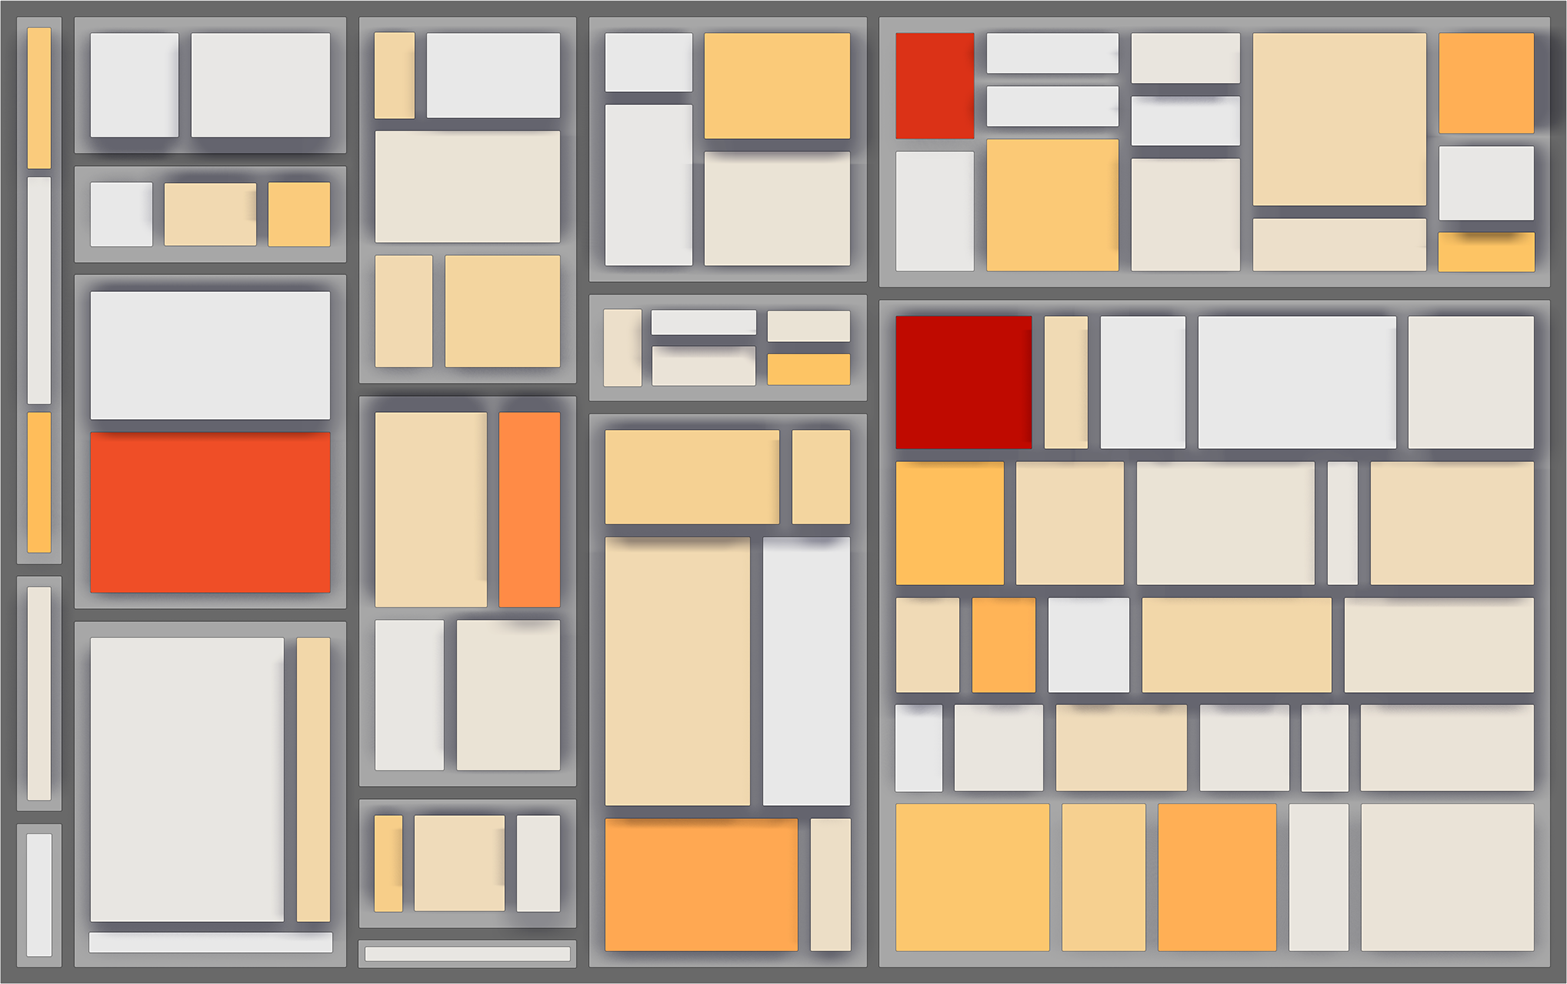
\includegraphics[width=1.0\linewidth]{figures/rectangular-map-wide.png}
	\caption{An example of a 2D treemap depicting software system data using area and color mapping as well as nesting.}
	\label{fig:treemap-example}
\end{figure}

\section{\uppercase{Foundation of Treemaps}}
\noindent%
For the last 30 years, the treemap visualization technique was extended, refined, and used in different contexts.
This adaptation process extended the scope of and expectations from treemaps for visualization designers and users.
Here, we want to recapitulate the original forces and predecessors leading to the first treemap visualization technique and introduce a conceptual visualization pipeline that seems common to all hierarchy visualization techniques.
Further, we review other generalization approaches for treemaps.

\paragraph{Predecessors of Treemaps.}
\label{sec:predecessors}
Upon looking back from the first mentioning of a treemap, the preceding ingredients for this visualization technique can be found in statistical cartograms, mosaic displays, and nested depiction for hierarchical components.
The early treemaps are a skilled combination of those techniques.
One original building block is the statistical cartogram~\cite{raisz1934-cartogram}.
These manually designed cartograms depicted geographic and demographic data by derivation of rectangular diagrams.
Thereby, adjacency of geographic locations were maintained and the rectangle for a location could be varied in size depending on the demographic data.
These properties are now backed by algorithms and attainable by IT systems as well~\cite{kreveld2007-rectangularcartograms}.
A second building block, the mosaic display~\cite{friendly2002-mosaicdisplay}, uses an algorithmic approach to dissect the surface for depiction.
The mosaic display appeared around 1877 and gained scientific attention in 1981.
The technique uses a two-dimensional subdivision of a rectangle based on categorical distribution for data points in two attributes---or more using scatter-plot techniques.
The main insights from those diagrams are the distribution of data items among different categories.
That is, treemaps were anecdotally referred to as \enquote{large weighted Venn diagrams}~\cite{johnson1993-categorical}.
A third building block is the depiction of hierarchical relations using nesting.
For example, they can be found with contour models~\cite{johnston1969-structure} and Nassi-Shneiderman-Diagrams~\cite{nassi1973-flowcharts}, used for depiction of hierarchical components of algorithms.
A combination of these approaches resulted in the first treemap visualization technique~\cite{johnson1991-spacefilling}.

\paragraph{Treemap Visualization Pipeline.}
\label{sec:pipeline}
We assume that the creation of visual representations from data, e.g., the transformation of tree-structured data into images from tree maps, can be understood as a visualization pipeline.
This pipeline can be a part of an interactive feedback loop of creating images from data, perceiving these images, and gaining insights---the visualization process (\autoref{fig:visualization-process}).
Within this process, the visualization pipeline is represented using three phases, namely \emph{Preprocessing}, \emph{Mapping}, and \emph{Image Synthesis}.
The required algorithms to create a treemap visualization from raw data are associated to one, or sometimes multiple, phases of this pipeline.
Thereby, some algorithms are specific to treemap visualization and others are more generally applicable in the fields of data processing and information visualization.
The specifics for treemap visualization techniques are prominent in the mapping phase and the geometry phase, i.e., these phases highly contribute to the appearance of a treemap visualization (\autoref{fig:pipeline}).
\begin{figure}[b]
	\centering
	

{
	\small
    \centering
    \begin{tikzpicture}
    \begin{scope}[node distance = 6pt]
    \node [data] (problemdata) {};
    \node [stagev] (analysis) [below=of problemdata,yshift=-1.2\baselineskip] {Analysis};
    \node [data] (visualizationdata) [below=of analysis] {};
    \node [stagev] (filtering) [below=of visualizationdata] {Preprocessing \& Filtering};
    \node [data] (focustree) [below=of filtering,xshift=10pt] {};
    \node [data] (focusdata) [below=of filtering,xshift=-10pt] {};
    \node [stagev] (layouting) [below=of focusdata,xshift=10pt,yshift=-1.2\baselineskip] {Layouting};
    \node [data] (layout) [below=of layouting] {};
    
    \node [stagev] (geometrycreation) [below=of layout] {Geometry Creation};
    \node [data] (geometry) [below=of geometrycreation] {};
    \node [stagev] (rendering) [below=of geometry,yshift=-1.1\baselineskip] {Rendering};
    \node [data] (image) [below=of rendering,yshift=-0.1\baselineskip] {};
    \end{scope}
    \connectfromdatav{problemdata}{analysis};
    \connecttodatav{analysis}{visualizationdata};
    \connectfromdatav{visualizationdata}{filtering};
    \connecttodatav{filtering}{focusdata};
    \connecttodatav{filtering}{focustree};
    \connectfromdatav{focusdata}{layouting};
    \connectfromdatav{focustree}{layouting};
    \connecttodatav{layouting}{layout};
    \connectfromdatav{layout}{geometrycreation};
    \connecttodatav{geometrycreation}{geometry};
    \connectfromdatav{geometry}{rendering};
    \connecttodatav{rendering}{image};
    \node (datalabel) [left=20pt of problemdata] {};
    \node at (datalabel.east) [text depth=0pt,xshift=0pt,anchor=east] {Problem Data};
    \draw [draw=black,very thin,shorten >= 0pt,shorten <= 3pt] (problemdata) -- (datalabel);
    \node (visdatalabel) [left=10pt of visualizationdata] {};
    \node at (visdatalabel.east) [text depth=0pt,xshift=0pt,anchor=east,text width=70pt,align=right] {Visualization Data};
    \draw [draw=black,very thin,shorten >= 0pt,shorten <= 3pt] (visualizationdata) -- (visdatalabel);
    \node (treelabel) [right=10pt of focustree] {};
    \node at (treelabel.west) [text depth=0pt,xshift=0pt,anchor=west] {Topology};
    \draw [draw=black,very thin,shorten >= 0pt,shorten <= 3pt] (focustree) -- (treelabel);
    \node (attributeslabel) [left=10pt of focusdata] {};
    \node at (attributeslabel.east) [text depth=0pt,xshift=0pt,anchor=east] {Attributes};
    \draw [draw=black,very thin,shorten >= 0pt,shorten <= 3pt] (focusdata) -- (attributeslabel);
    \node (layoutlabel) [left=10pt of layout] {};
    \node at (layoutlabel.east) [text depth=0pt,xshift=0pt,anchor=east] {Layout};
    \draw [draw=black,very thin,shorten >= 0pt,shorten <= 3pt] (layout) -- (layoutlabel);
    \node (geometrylabel) [left=10pt of geometry] {};
    \node at (geometrylabel.east) [text depth=0pt,xshift=0pt,anchor=east] {Geometry};
    \draw [draw=black,very thin,shorten >= 0pt,shorten <= 3pt] (geometry) -- (geometrylabel);
    \node (imagelabel) [left=20pt of image] {};
    \node at (imagelabel.east) [text depth=0pt,xshift=0pt,anchor=east] {Image};
    \draw [draw=black,very thin,shorten >= 0pt,shorten <= 3pt] (image) -- (imagelabel);
    \begin{scope}[on background layer]
    \node [phasev,phasename=Preprocessing] (preprocessing) [fit={(analysis)(filtering)($(analysis.north)+(0pt,1.0\baselineskip)$)}] {};
    \node [phasev,phasename=Mapping] (mapping) [fit={(layouting)(geometrycreation)($(layouting.north)+(0pt,1.0\baselineskip)$)}] {};
    \node [phasev,phasename=Image Synthesis] (imagesynthesis) [fit={(rendering)($(rendering.north)+(0pt,1.0\baselineskip)$)}] {};
    \node [pipeline] (pipeline) [fit={(preprocessing.north)(preprocessing.west)(imagesynthesis.east)(imagesynthesis.south)}] {};
    \end{scope}
    \end{tikzpicture}
}

	\caption{Concept of a hierarchy visualization pipeline including the tree structure (topology), per-node attributes, and the spatialization process of this abstract data.}
	\label{fig:pipeline}
\end{figure}
\begin{figure*}[t]
	\centering
	

{%
	\small
	\linespread{0.8}
    \centering
    \begin{tikzpicture}
    \begin{scope}[node distance = 27pt,every node/.style={inner sep=0,outer sep=0}]
    \node [data] (problemdata) {};
    \node [phase,text width=60pt,align=center,text depth=0pt] (preprocessing) [right=of problemdata] {Preprocessing};
    \node [data] (focusdata) [right=of preprocessing] {};
    \node [smalldata] (preprocessing-config) [below=8pt of preprocessing] {};
    \node [phase,align=center] (mapping) [right=of focusdata,text depth=0pt] {Mapping};
    \node [data] (geometry) [right=of mapping] {};
    \node [smalldata] (mapping-config) [below=8pt of mapping] {};
    \node [phase,align=center] (imagesynthesis) [right=of geometry,text depth=0pt] {Image Synthesis};
    \node [data] (image) [right=of imagesynthesis] {};
    \node [smalldata] (imagesynthesis-config) [below=8pt of imagesynthesis] {};
    \node [phase,text width=60pt,align=center,yshift=-4pt] (perception) [below=of imagesynthesis,text depth=1.2\baselineskip] {Perception \& Cognition}; %
    \node [data] (knowledge) [left=of perception] {};
    \node [phase,align=center] (exploration) [left=of knowledge,text depth=0pt] {Exploration};
    \node [data] (config) [left=of exploration] {};
    \node [phase,align=center] (api) [left=of config] {API};
    \end{scope}
    \connectfromdata{problemdata}{preprocessing};
    \connecttodata{preprocessing}{focusdata};
    \connectionSmallN{preprocessing-config}{preprocessing-config-center};
    \draw[draw=black,very thin] (preprocessing-config-center.center) -- (preprocessing);
    \connectfromdata{focusdata}{mapping};
    \connecttodata{mapping}{geometry};
    \connectionSmallN{mapping-config}{mapping-config-center};
    \draw[draw=black,very thin] (mapping-config-center.center) -- (mapping);
    \connectfromdata{geometry}{imagesynthesis};
    \connecttodata{imagesynthesis}{image};
    \connectionSmallN{imagesynthesis-config}{imagesynthesis-config-center};
    \draw[draw=black,very thin] (imagesynthesis-config-center.center) -- (imagesynthesis);
    \connectionS{image}{imagecenter};
    \draw[draw=black,very thin] (imagecenter.center) |- (perception) node[pos=0.75] (perceptionloop-join) {};
    \draw[draw=black,very thin] (perception.west) -- (knowledge.east);
    \connectionW{knowledge}{knowledgecenter};
    \draw[draw=black,very thin] (knowledgecenter.center) -- (exploration) node[pos=0.5] (perceptionloop-split) {};
    \draw[draw=black,very thin] (exploration.west) -- (config.east);
    \draw[draw=black,very thin,->] (perceptionloop-split.center) -- ($(perceptionloop-split)+(0pt,-16pt)$) -- ($(perceptionloop-join)+(0pt,-16pt)$) -- (perceptionloop-join.center);
    \connectionW{config}{configcenter};
    \draw[draw=black,very thin] (configcenter.center) -- (api);
    \draw[draw=black,very thin] (api) -- (preprocessing-config) node[pos=0.90] (preprocessing-config-split) {};
    \draw[draw=black,very thin] (preprocessing-config-split.center) -| (mapping-config) node[pos=0.5] (mapping-config-split) {};
    \draw[draw=black,very thin] (mapping-config-split.center) -| (imagesynthesis-config);
    \node[above=6pt of problemdata,align=center] (problemdatalabel) {Problem Data};
    \draw [draw=black,very thin,shorten >= -1pt,shorten <= 2pt] (problemdata) -- (problemdatalabel);
    \node[above=6pt of focusdata,align=center] (focusdatalabel) {Focus Data};
    \draw [draw=black,very thin,shorten >= -1pt,shorten <= 2pt] (focusdata) -- (focusdatalabel);
    \node[above=6pt of geometry,align=center,text depth=0pt] (geometrylabel) {Geometry};
    \draw [draw=black,very thin,shorten >= -1pt,shorten <= 2pt] (geometry) -- (geometrylabel);
    \node[above=6pt of image,align=center] (imagelabel) {Image};
    \draw [draw=black,very thin,shorten >= -1pt,shorten <= 2pt] (image) -- (imagelabel);
    \node[above=6pt of knowledge,align=center,text depth=0pt] (knowledgelabel) {Knowledge};
    \draw [draw=black,very thin,shorten >= -1pt,shorten <= 2pt] (knowledge) -- (knowledgelabel);
    \node[above=6pt of config,align=center,text depth=0pt] (configlabel) {Configuration};
    \draw [draw=black,very thin,shorten >= -1pt,shorten <= 2pt] (config) -- (configlabel);
    \begin{scope}[on background layer]
    \node [pipeline,pipelinename=Visualization Pipeline,fill=gray!8] (pipeline) [fit={($(preprocessing.north)+(0pt,1.2\baselineskip)$)(preprocessing.west)(imagesynthesis.east)(imagesynthesis.south)}] {};
    \node [pipeline,pipelinename=User,fill=gray!8] (user) [fit={($(exploration.north)+(0pt,1.2\baselineskip)$)(exploration.west)(perception.east)(perception.south)}] {};
    \end{scope}
    \end{tikzpicture}%
}%

	\caption{%
		Illustration of the visualization process and the included visualization pipeline.
		Adapted from van Wijk (2005).%
	}
	\label{fig:visualization-process}
\end{figure*}
	
\paragraph{Generalization on Treemaps.}
\label{sec:generalization}
The similarities of treemap visualizations, as proposed by Shneiderman and Johnson, to other hierarchy visualization techniques were used before to provide means of generalization of hierarchy visualization techniques.
As such, Schulz et~al. coined the term implicit hierarchy visualizations~\cite{schulz2011-implicit} as a category of visualization techniques that uses implicit, i.e., non-drawn, metaphors to represent the parent-child relationships.
Later, Schulz et~al. presented a generative layout approach for rooted tree drawings that could be used to create a wide range (and mixed use) of visualization techniques with implicit and explicit edge representations~\cite{schulz2013-generativelayout}.
Likewise, Baudel and Broeksema discussed a design space for rectangular, sequential, and space-filling treemap layouts~\cite{baudel2012-designspace}, creating an own set of treemap visualization techniques.

\begin{figure*}[t]%
	\centering
	

{%
	\footnotesize
	\centering%
	\newlength{\definitionswidth}%
	\newlength{\definitionsoffset}%
	\newlength{\definitionsimagesize}%
	\newlength{\definitionsdescriptionsize}%
	\setlength{\definitionswidth}{\textwidth}%
	\setlength{\definitionsoffset}{13pt}%
	\setlength{\definitionsimagesize}{0.25\definitionswidth - 2\definitionsoffset}%
	\setlength{\definitionsdescriptionsize}{0.25\definitionswidth - 0.5\definitionsoffset}%
	\begin{tikzpicture}[]
	\node[inner sep=0,outer sep=0] (space-filling) at (-1.5\definitionsimagesize - 3\definitionsoffset, 0.0) {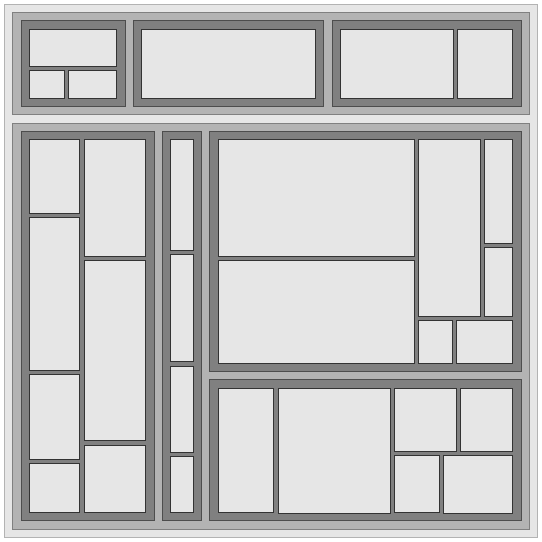
\includegraphics[width=\definitionsimagesize]{figures/treemap-cat-s}};
	\node[inner sep=0,outer sep=0] (containment) at (-0.5\definitionsimagesize + -1\definitionsoffset, 0.0) {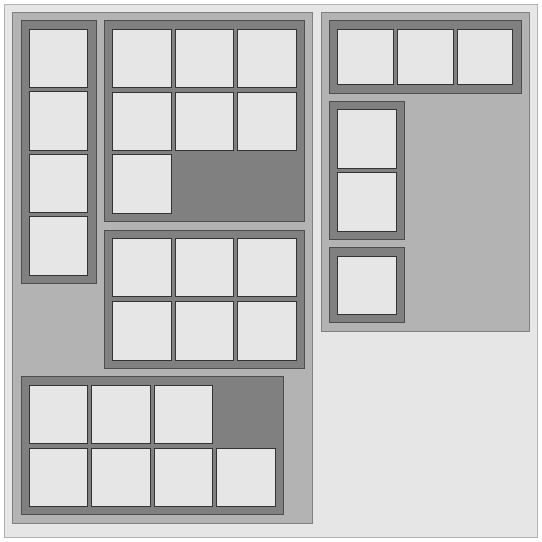
\includegraphics[width=\definitionsimagesize]{figures/treemap-cat-c}};
	\node[inner sep=0,outer sep=0] (implicit-edge) at (0.5\definitionsimagesize + 1\definitionsoffset, 0.0) {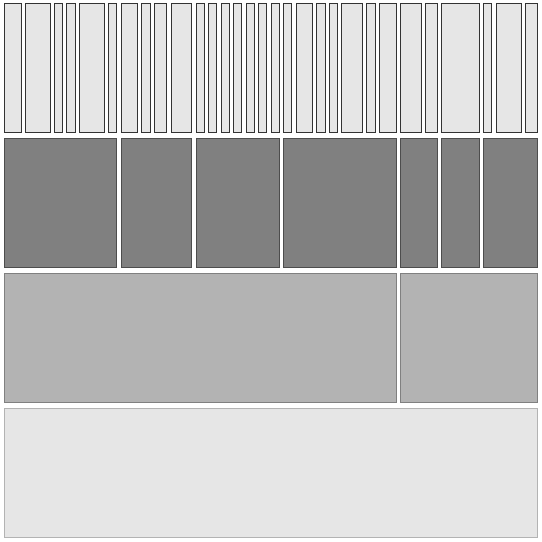
\includegraphics[width=\definitionsimagesize]{figures/treemap-cat-ie}};
	\node[inner sep=0,outer sep=0] (mapped-tree) at (1.5\definitionsimagesize + 3\definitionsoffset, 0.0) {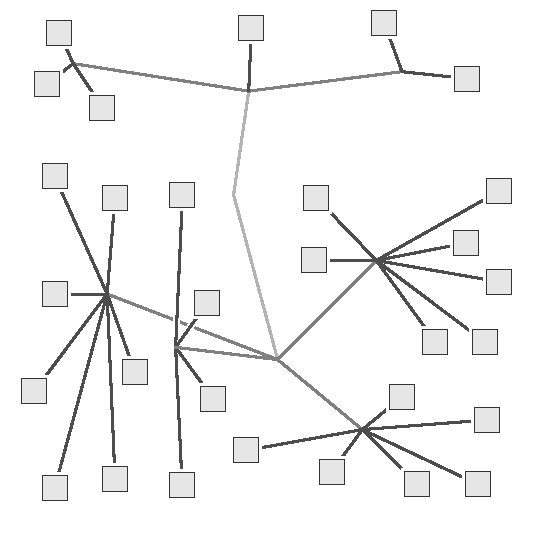
\includegraphics[width=\definitionsimagesize]{figures/treemap-cat-mt}};
	\node[above=0cm of space-filling] (tm0) {\Ts};
	\node[below=0cm of space-filling,text width=\definitionsdescriptionsize,align=center] (tm0-description) { Space-filling Treemap };
	\node[above=0cm of containment] (tm1) {\Tc};
	\node[below=0cm of containment,text width=\definitionsdescriptionsize,align=center] (tm1-description) { Containment Treemap };
	\node[above=0cm of implicit-edge] (tm2) {\Tie};
	\node[below=0cm of implicit-edge,text width=\definitionsdescriptionsize,align=center] (tm2-description) { Implicit Edge Representation Tree };
	\node[above=0cm of mapped-tree] (tm3) {\Tmt};
	\node[below=0cm of mapped-tree,text width=\definitionsdescriptionsize,align=center] (tm3-description) { Mapped Tree };
	\draw[draw=none] (space-filling.east) -- (containment.west) node[pos=0.5] {\huge $\subset$};
	\draw[draw=none] (containment.east) -- (implicit-edge.west) node[pos=0.5] (splitting-subset) {\huge $\subset$};
	\draw[draw=none] (implicit-edge.east) -- (mapped-tree.west) node[pos=0.5] {\huge $\subset$};
	\draw[draw=none] (containment.center) -- (splitting-subset.center) node [pos=0.85] (discriminator-x) {};
	\draw[densely dotted,line width=0.75pt,shorten <= 5pt,shorten >= 5pt] (discriminator-x |- tm2.north) -- (discriminator-x |- tm2-description.south);
	\end{tikzpicture}%
}%

	\caption{The four proposed treemap categories, namely \emph{Space-filling Treemap}, \emph{Containment Treemap}, \emph{Implicit Edge Representation Tree}, and \emph{Mapped Tree}. Each category includes their predecessors, building a more general category. The dotted line highlights the observed current border, whether a visualization technique is called a treemap.}%
	\label{fig:treemap-categories}
\end{figure*}
\section{\uppercase{Categories}}
\label{sec:treemapcategories}%
\noindent
Throughout the community of information visualization, there seems to be some consensus on the visualization techniques that may be called a \emph{treemap}.
Disregarding their differences, the emerged set of common characteristics is as follows:
\begin{itemize}
	\setlength{\itemsep}{0pt}
	\item First, a treemap is a visualization technique suitable to depict tree-structured data.
	\item There is a representation of the parent-child relationships without use of explicit edge links, i.e., the containment metaphor~\cite{schulz2011-implicit}.
	\item The depiction of leaf nodes implies an area or volume in the geometry space~\cite{park2018-atomgrammar}.
	\item The representation of sibling nodes should be guaranteed to be non-overlapping~\cite{johnson1991-spacefilling}.
\end{itemize}
In other words, the prominent property for treemaps is the visual containment in the depiction, which implies a containment within the layout as well.
Empirically, the technique in question allows for at least one of either area, volume, or color for attribute mapping of leaf nodes.
More effective treemap visualization techniques allow for at least two visual variables for attribute mapping of leaf nodes.
\par
Based upon this, we believe the term \emph{treemap} is not only suitable for the first treemap introduced by Shneiderman and Johnson but for a broader range of hierarchy visualization techniques.
To contribute to the discussion, we propose four different sets of characteristics that could be used to distinguish between treemaps, tree visualization techniques, and general hierarchy visualization techniques (\Th):
\begin{itemize}
	\setlength{\itemsep}{0pt}
	\item the \emph{Space-filling Treemap}~\Ts,
	\item the \emph{Containment Treemap}~\Tc,
	\item the \emph{Implicit Edge Representation Tree}~\Tie,
	\item and the \emph{Mapped Tree}~\Tmt.
\end{itemize}
These categories focus on the characteristics of the spatialization process (resulting in the layout) and the visual representation in geometry space.
Thereby, each category is a superset of the previous one, forming a hierarchy of tree visualization techniques.
This property allows to categorize the taxonomy itself as a hyponymy.
The four categories are motivated and defined as follows.
\newlength{\treemapinsetdefaultwidth}
\setlength{\treemapinsetdefaultwidth}{0.24\linewidth} %
\par
\begin{wrapfigure}{r}{\treemapinsetdefaultwidth}%
	\vspace{-1.4\baselineskip}
	\begin{tikzpicture}[]
	\node[inner sep=0,outer sep=0] (spacefilling) at (0,0) {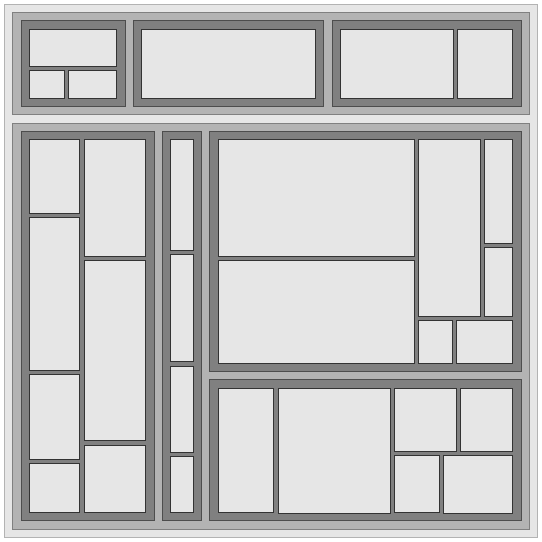
\includegraphics[width=\treemapinsetdefaultwidth]{figures/treemap-cat-s}};
	\node[above=0cm of spacefilling] (Ts) {\Ts};
	\draw[thin,black,shorten >= 6pt] (Ts-|spacefilling.west) -- (Ts);
	\draw[thin,black,shorten <= 6pt] (Ts) -- (Ts-|spacefilling.east);
	\end{tikzpicture}
	\vspace{-1.6\baselineskip}
\end{wrapfigure}%
\paragraph{Space-filling Treemap.}%
A space-filling treemap results from a recursive subdivision of a surface~\cite{johnson1991-spacefilling} or an $n$-dimensional cube~\cite{johnson1993-categorical}.
The main characteristic is the full subdivision and distribution of a parents' surface or volume for its children, resulting in space-filling depictions of the leaf nodes.
This category of treemaps includes not only subdivisions of rectangles but others as general rectangular~\cite{wattenberg2005-spacefillingcurves}, convex polygonal~\cite{balzer2005-voronoi,wang2019-orthogonalvoronoi}, and non-convex polygonal~\cite{auber2013-gospermap} partitions as well (\autoref{fig:TM0-examples}).

\par
\begin{wrapfigure}{r}{\treemapinsetdefaultwidth}%
	\vspace{-1.4\baselineskip}
	\begin{tikzpicture}[]
	\node[inner sep=0,outer sep=0] (containment) at (0,0) {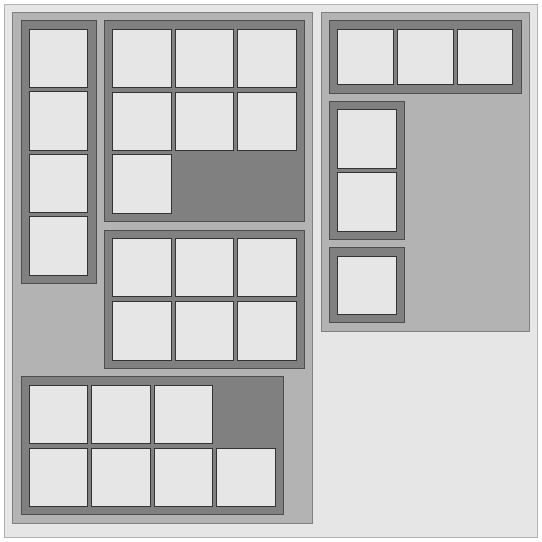
\includegraphics[width=\treemapinsetdefaultwidth]{figures/treemap-cat-c}};
	\node[above=0cm of containment] (Tc) {\Tc};
	\draw[thin,black,shorten >= 6pt] (Tc-|containment.west) -- (Tc);
	\draw[thin,black,shorten <= 6pt] (Tc) -- (Tc-|containment.east);
	\end{tikzpicture}
	\vspace{-1.6\baselineskip}
\end{wrapfigure}%
\paragraph{Containment Treemap.}%
The category of \emph{Containment Treemaps} extends \emph{Space-filling Treemaps} by loosening the space-filling property.
This still requires that child nodes are located within their parent surfaces but they must not utilize all the space of the parent.
Mainly, hierarchy visualization techniques from this category are currently considered treemap visualization techniques.
Typically, the corresponding layouts are created using packing algorithms~\cite{yamaguchi2003-datajewelry,wettel2008-large,scheibel2018-evocells} (\autoref{fig:TM1-examples}).
Another approach is the transformation of the treemap layout, e.g. for Generalized Treemaps~\cite{vliegen2006-businessdata}.
Similarly to space-filling treemaps, containment treemaps allow for different geometrical shapes as well, e.g., circles~\cite{wetzel2003-pebbles,gortler2017-bubbletreemaps} and ellipses~\cite{otjacques2007-ellimaps}.

\par
\begin{wrapfigure}{r}{\treemapinsetdefaultwidth}%
	\vspace{-1.4\baselineskip}
	\begin{tikzpicture}[]
	\node[inner sep=0,outer sep=0] (implicitedge) at (0,0) {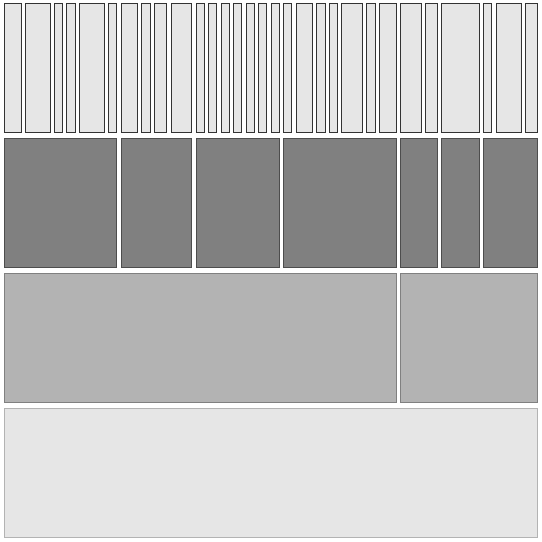
\includegraphics[width=\treemapinsetdefaultwidth]{figures/treemap-cat-ie}};
	\node[above=0cm of implicitedge] (Tie) {\Tie};
	\draw[thin,black,shorten >= 6pt] (Tie-|implicitedge.west) -- (Tie);
	\draw[thin,black,shorten <= 6pt] (Tie) -- (Tc-|implicitedge.east);
	\end{tikzpicture}
	\vspace{-1.6\baselineskip}
\end{wrapfigure}%
\paragraph{Implicit Edge Representation Tree.}%
When loosening the containment property and allowing all types of implicit edge representations~\cite{schulz2011-implicit}, i.e., containment, adjacency, and overlap, an even broader set of visualization techniques can be labeled as \emph{treemaps}.
With this set of characteristics, visualization techniques that were created using transformations on treemap layouts, e.g., \emph{Cascaded Treemaps}~\cite{lu2008-cascadedtreemaps} and the \emph{BeamTree}~\cite{vanHam2003-beamtrees}, can be considered treemaps as well.
In fact, their goal is to \enquote{convey the same containment relationship}~\cite{lu2008-cascadedtreemaps} and effectively do so.
Applying the idea of layout postprocessings to one-dimensional treemap layouts, the results are icicle plots~\cite{kruskal1983-icicle}, and with additional projection they can result in sunburst views~\cite{stasko2000-structures}, and other derived techniques~\cite{webber2006-space,holten2006-edgebundles} (\autoref{fig:TM2-examples}).
This is valid as implicit edge representations fulfill the \emph{containment property} during layouting as well but the depiction in geometry space may drop the visual cues for containment~\cite{johnson1993-categorical}.

\par
\begin{wrapfigure}{r}{\treemapinsetdefaultwidth}%
	\vspace{-1.4\baselineskip}
	\begin{tikzpicture}[]
	\node[inner sep=0,outer sep=0] (mappedtree) at (0,0) {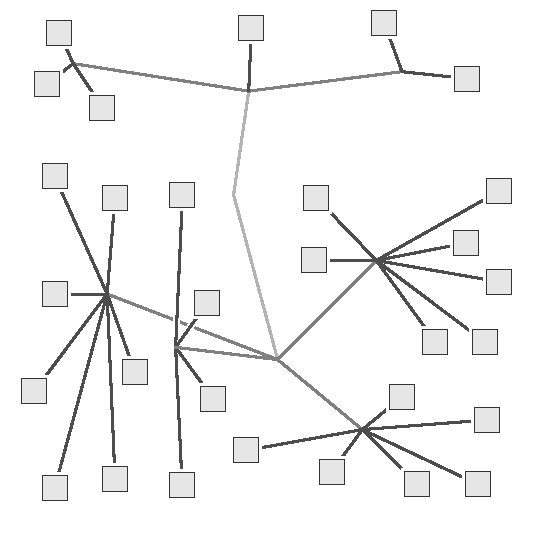
\includegraphics[width=\treemapinsetdefaultwidth]{figures/treemap-cat-mt}};
	\node[above=0cm of implicitedge] (Tmt) {\Tmt};
	\draw[thin,black,shorten >= 6pt] (Tmt-|mappedtree.west) -- (Tmt);
	\draw[thin,black,shorten <= 6pt] (Tmt) -- (Tmt-|mappedtree.east);
	\end{tikzpicture}
	\vspace{-1.6\baselineskip}
\end{wrapfigure}%
\paragraph{Mapped Tree.}%
While all previously proposed categories use an implicit edge representation, there are tree visualization techniques that use other relation encoding techniques such as vicinity or explicit links~\cite{schulz2013-generativelayout}.
Most of them share the invariant of overlap-free spatialization across node siblings, resulting in an unambiguous bidirectional mapping of the tree-structure to the depiction.
Such a depiction is provided if the underlying tree layout is based on the property of containment, even if the resulting visualization does not encode the parent-child relationship using an implicit edge representation.
Exemplary visualization techniques for the \emph{Mapped Tree} category include space-optimized trees~\cite{nguyen2002-sot}, contour maps~\cite{kubota2006-visualization}, and point-based tree depictions~\cite{schulz2011-pointbased} (\autoref{fig:TM3-examples}).
Assuming a bidirectional mapping of layout algorithms, \enquote{[c]ontainment based treemap algorithms [\ldots] form the core of a powerful and extensible grand unified theory of hierarchical visualization---the treemap}~\cite{johnson1993-categorical}.

\begin{table}[b]
	\centering
	\scriptsize
	\noindent%
	\setlength{\tabcolsep}{0.75pt}%
	\renewcommand{\arraystretch}{1.03}%
	\rowcolors{1}{white}{gray!10}%
	\caption{%
		An association of different hierarchy visualization techniques to the proposed taxonomy.
		For direct comparison, this table includes hierarchy visualization techniques \Th{} that are not covered by this taxonomy as well.
		The \OKbf{} and \OK{} dots denote the most specific category and associated hyperonyms (more general categories), respectively.%
		\vspace{0.5em}%
	}%
	\label{tab:association}
	\begin{tabularx}{\linewidth}{@{}X|cccc|c@{}}
		\toprule
		\textbf{Visualization Technique} & \Ts  & \Tc & \Tie & \Tmt & \Th \\
		\midrule
		BeamTree~\cite{vanHam2003-beamtrees} & & & \OKbf & \OK & \OK
		\\ Bundle View~\cite{holten2006-edgebundles} & & & \OKbf & \OK & \OK
		\\ Cactus Tree~\cite{dang2017-cactustree} & & & & & \OKbf
		\\ CodeCity~\cite{wettel2008-large} & & \OKbf & \OK & \OK & \OK
		\\ Contrast Treemaps~\cite{tu2007-changes} & \OKbf & \OK & \OK & \OK & \OK
		\\ Data Jewelry Box~\cite{itoh2004-reactanglepacking} & & \OKbf & \OK & \OK & \OK
		\\ Ellimaps~\cite{otjacques2007-ellimaps} & \OKbf & \OK & \OK & \OK & \OK
		\\ EvoCells~\cite{scheibel2018-evocells} & & \OKbf & \OK & \OK & \OK
		\\ Flame Graph~\cite{gregg2016-flamegraphs} & & & \OKbf & \OK & \OK
		\\ Gosper Map~\cite{auber2013-gospermap} & \OKbf & \OK & \OK & \OK & \OK
		\\ Icicle Plot~\cite{kruskal1983-icicle} & & & \OKbf & \OK & \OK
		\\ Information Slices~\cite{andrews1998-slices} & & & & \OKbf & \OK
		\\ Overlap-free Pythagoras Tree~\cite{munz2019-pythagorastrees} & & & & \OKbf & \OK
		\\ Pebbles Treemap~\cite{wetzel2003-pebbles} & & \OKbf & \OK & \OK & \OK
		\\ Pythagoras Tree~\cite{beck2014-pythagorastrees} & & & & & \OKbf
		\\ Quantum Treemaps~\cite{bederson2002-quantum} & & \OKbf & \OK & \OK & \OK
		\\ Slice'n'Dice Treemap~\cite{johnson1991-spacefilling} & \OKbf & \OK & \OK & \OK & \OK
		\\ Software Cities~\cite{steinbruckner2013-evolution} & & & & \OKbf & \OK
		\\ Space-Optimized Tree~\cite{nguyen2002-sot} & & & & \OKbf & \OK
		\\ Stable Voronoi Treemap~\cite{hahn2013-varyinghierarchies} & \OKbf & \OK & \OK & \OK & \OK
		\\ Sunburst View~\cite{stasko2000-structures} & & & \OKbf & \OK & \OK
		\\ Tree Drawings~\cite{toosi2014-circular} & & & & \OKbf & \OK
		\\ Treemaps with Bound Aspect Ratio~\cite{deBerg2011-bounded} & \OKbf & \OK & \OK & \OK & \OK
		\\ Voronoi Treemap~\cite{balzer2005-softwaremetrics} & \OKbf & \OK & \OK & \OK & \OK
		\\ \bottomrule
	\end{tabularx}
\end{table}

\newlength{\examplesdefaultwidth}
\setlength{\examplesdefaultwidth}{0.1815\textwidth} %
\begin{figure*}[p]
	\centering
	\footnotesize
	\begin{tikzpicture}[every node/.style={inner sep=0,outer sep=0},node distance=0pt]
	\node[] (sot-1) {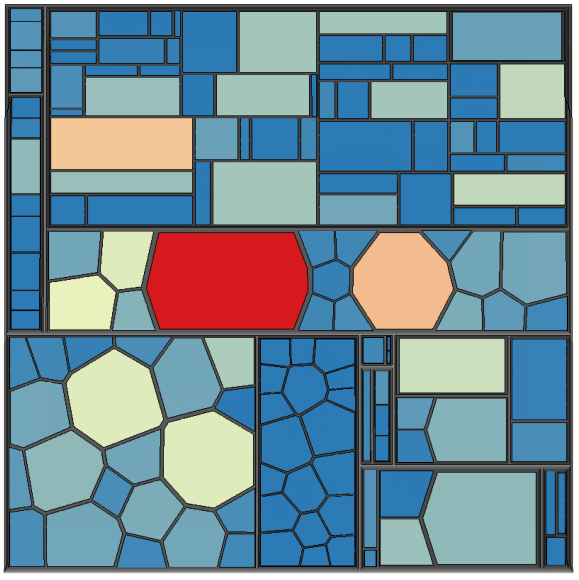
\includegraphics[width=\examplesdefaultwidth]{figures/mixed-treemap-layouting.png}};
	\node[below=5pt of sot-1,text width=\examplesdefaultwidth,align=center] (sot-1-label) { Hybrid Layout Treemap };
	\node[right=10pt of sot-1] (sot-2) {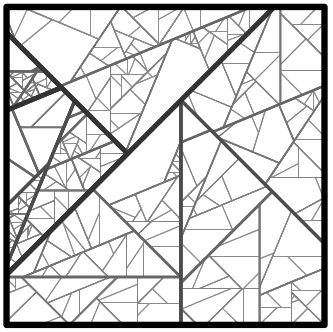
\includegraphics[width=\examplesdefaultwidth]{figures/bound-aspect-ratio.png}};
	\node[below=5pt of sot-2,text width=\examplesdefaultwidth,align=center] (sot-2-label) { Treemap with Bound Aspect Ratio };
	\node[right=10pt of sot-2] (sot-3) {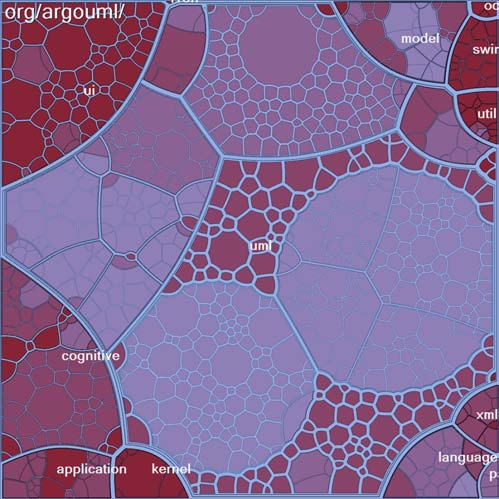
\includegraphics[width=\examplesdefaultwidth]{figures/voronoitreemap.png}};
	\node[below=5pt of sot-3,text width=\examplesdefaultwidth,align=center] (sot-3-label) { Voronoi Treemap };
	\node[right=10pt of sot-3] (sot-4) {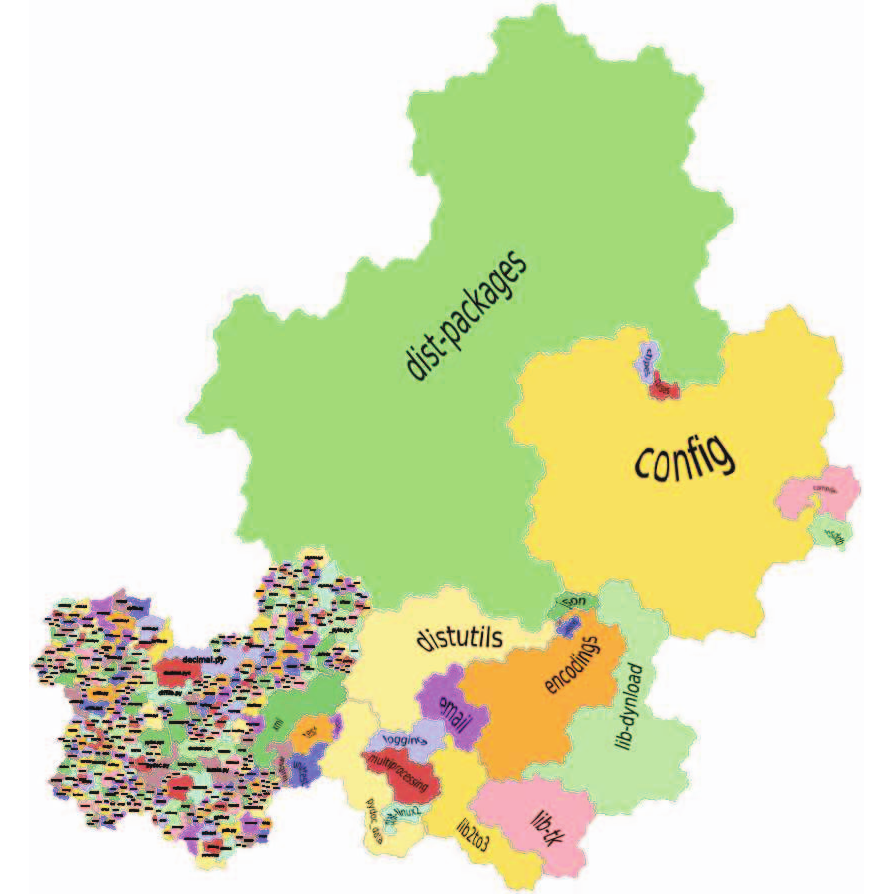
\includegraphics[width=\examplesdefaultwidth]{figures/gospermap.png}};
	\node[below=5pt of sot-4,text width=\examplesdefaultwidth,align=center] (sot-4-label) { GosperMap };
	\node[right=10pt of sot-4] (sot-5) {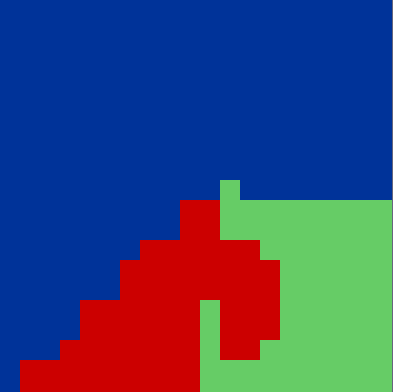
\includegraphics[width=\examplesdefaultwidth]{figures/jigsaw.png}};
	\node[below=5pt of sot-5,text width=\examplesdefaultwidth,align=center] (sot-5-label) { Jigsaw Treemap };
	\node[above=5pt of sot-3] (Ts) { \Ts };
	\draw[thin,black,shorten >= 10pt] (Ts-|sot-1.west) -- (Ts);
	\draw[thin,black,shorten <= 10pt] (Ts) -- (Ts-|sot-5.east);
	\end{tikzpicture}
	\caption{Examples of treemaps from the category \emph{Space-Filling Treemap}. Image courtesy from left to right: \cite{hahn2017-hybrid}, \cite{deBerg2011-bounded}, \cite{balzer2005-softwaremetrics}, \cite{auber2013-gospermap}, and \cite{wattenberg2005-spacefillingcurves}.}
	\label{fig:TM0-examples}
\end{figure*}
\begin{figure*}[p]
	\centering
	\footnotesize
	\begin{tikzpicture}[every node/.style={inner sep=0,outer sep=0},node distance=0pt]
	\node[] (sot-1) {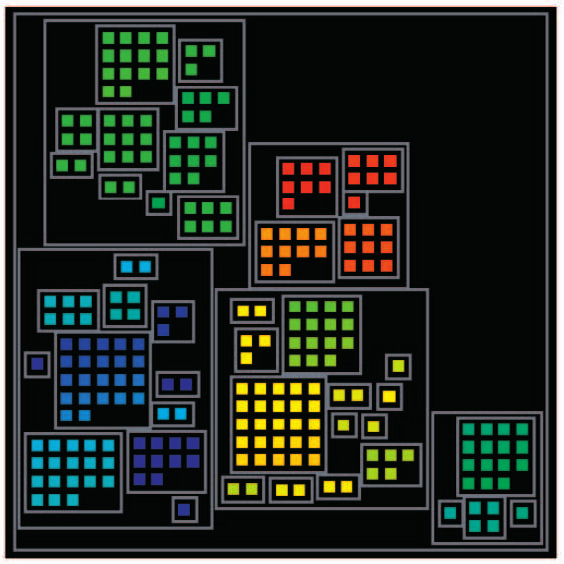
\includegraphics[width=\examplesdefaultwidth]{figures/data-jewelry-box.png}};
	\node[below=5pt of sot-1,text width=\examplesdefaultwidth,align=center] (sot-1-label) { Data-Jewelry Box };
	\node[right=10pt of sot-1] (sot-2) {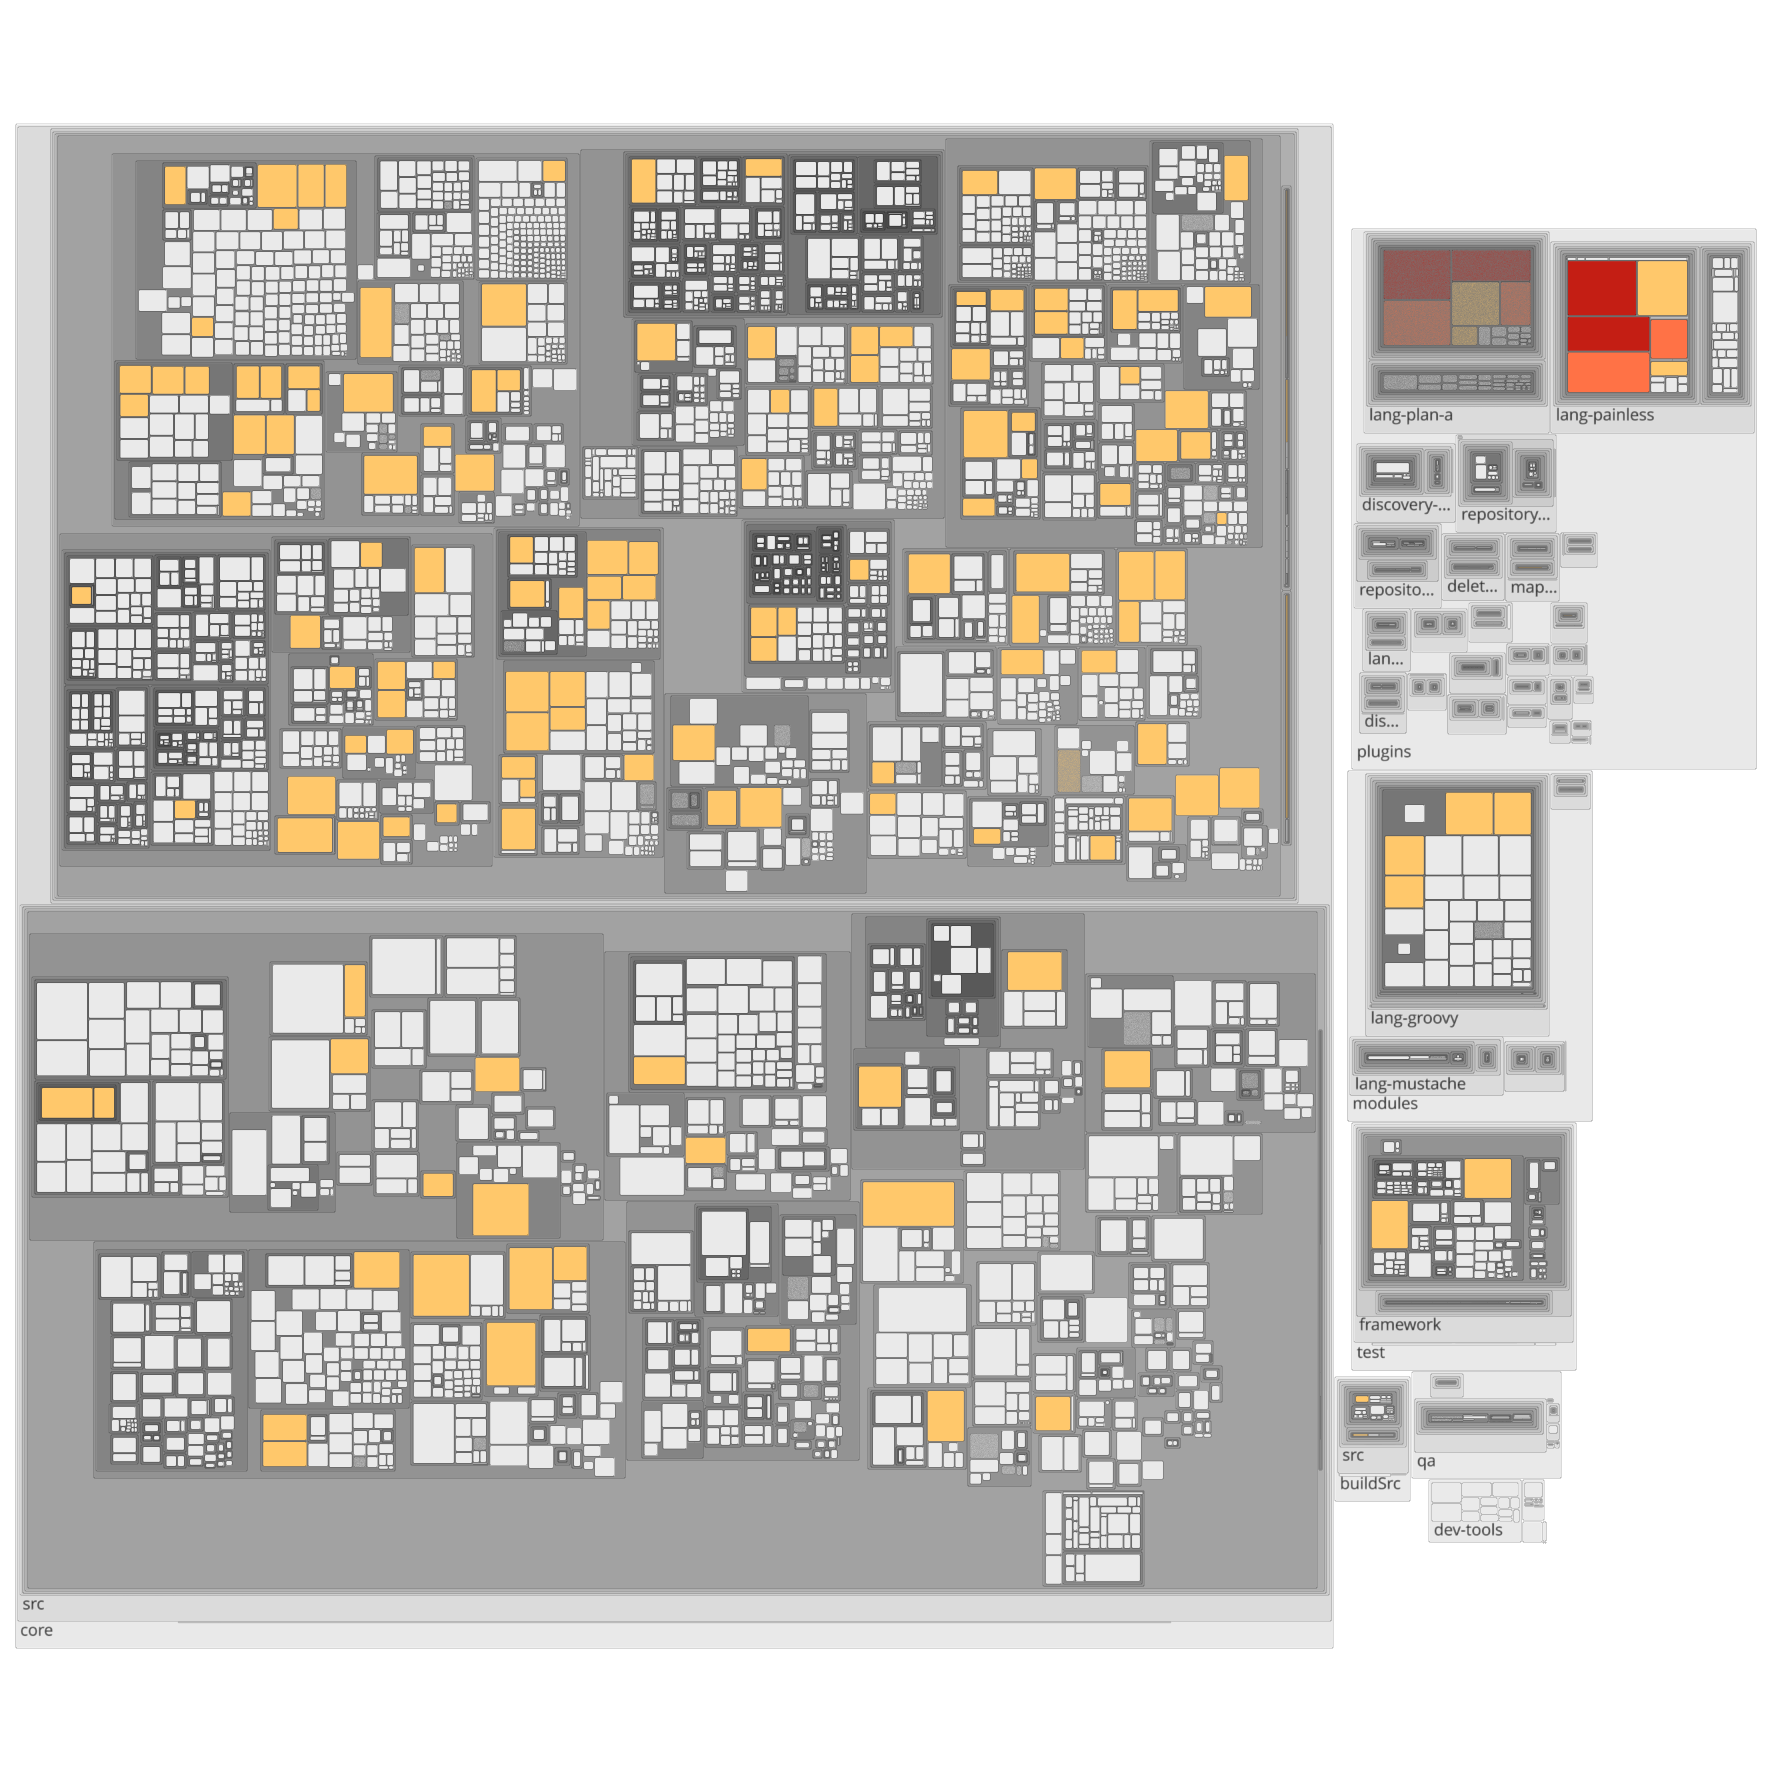
\includegraphics[width=\examplesdefaultwidth]{figures/evocells.png}};
	\node[below=5pt of sot-2,text width=\examplesdefaultwidth,align=center] (sot-2-label) { EvoCells Treemap };
	\node[right=10pt of sot-2] (sot-3) {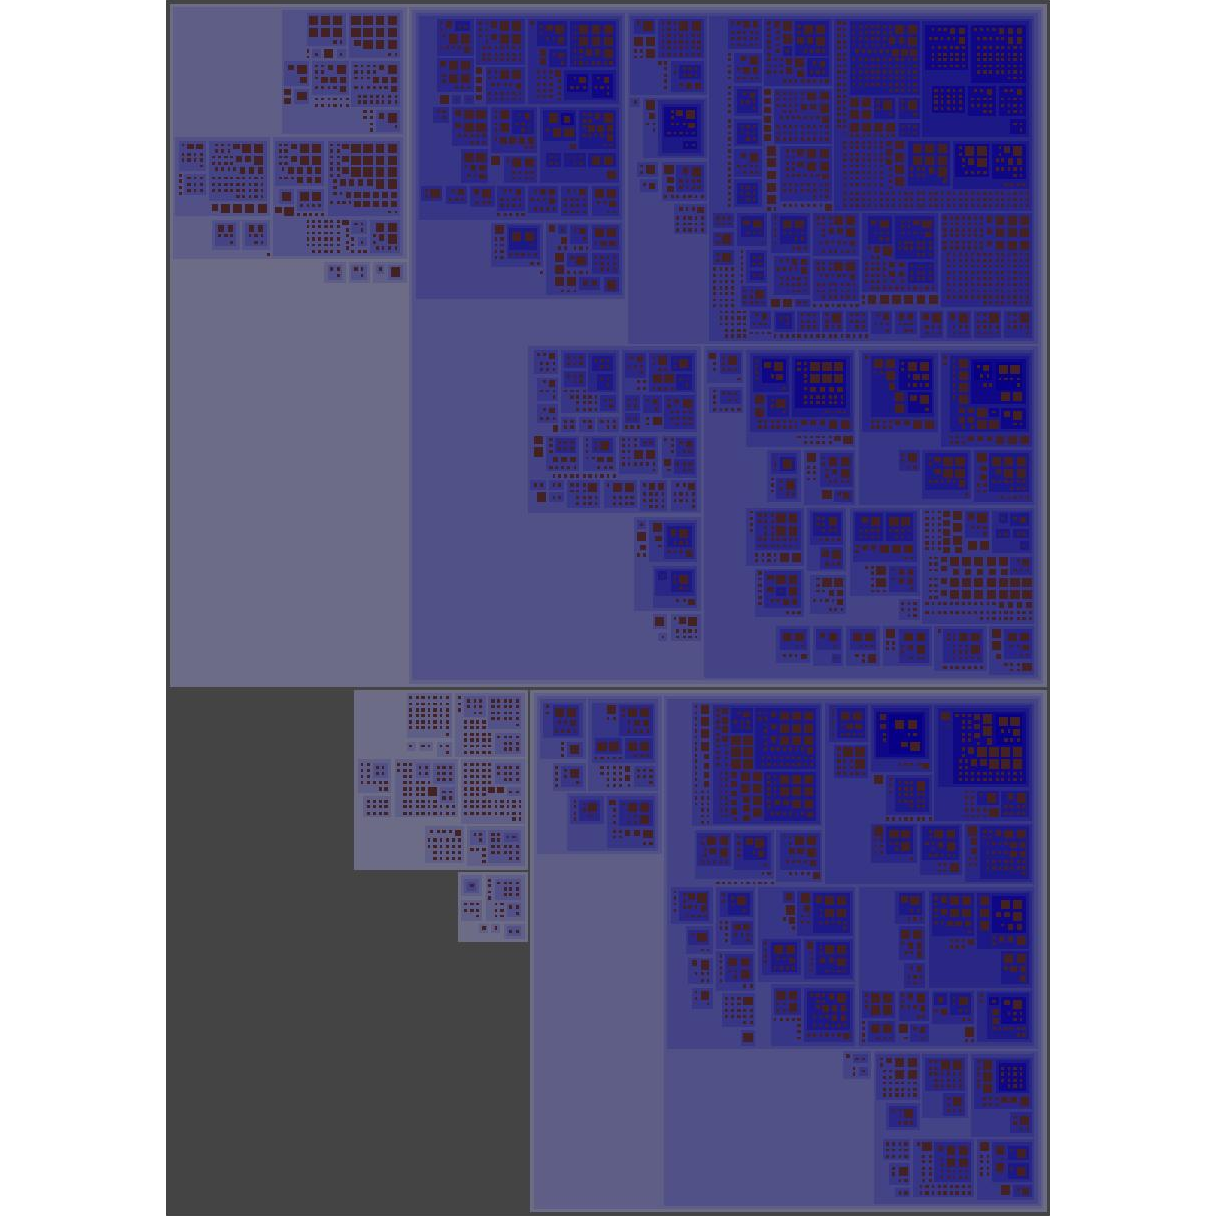
\includegraphics[width=\examplesdefaultwidth]{figures/codecity.png}};
	\node[below=5pt of sot-3,text width=\examplesdefaultwidth,align=center] (sot-3-label) { CodeCity };
	\node[right=10pt of sot-3] (sot-4) {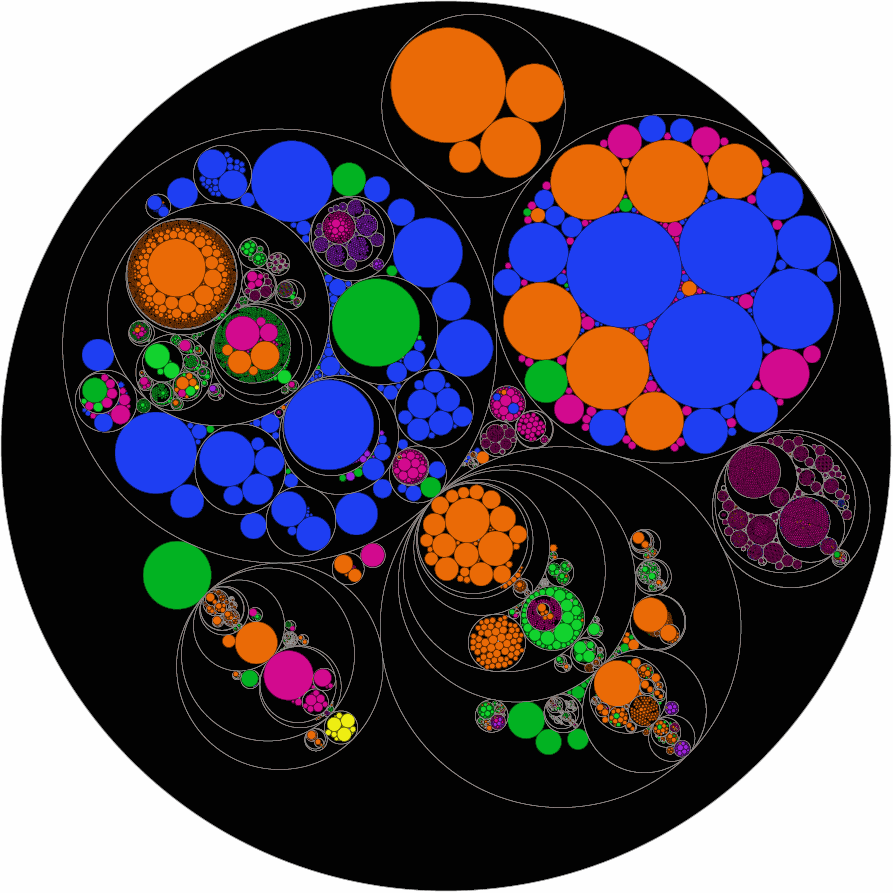
\includegraphics[width=\examplesdefaultwidth]{figures/pebbles.png}};
	\node[below=5pt of sot-4,text width=\examplesdefaultwidth,align=center] (sot-4-label) { Pebbles Treemap };
	\node[right=10pt of sot-4] (sot-5) {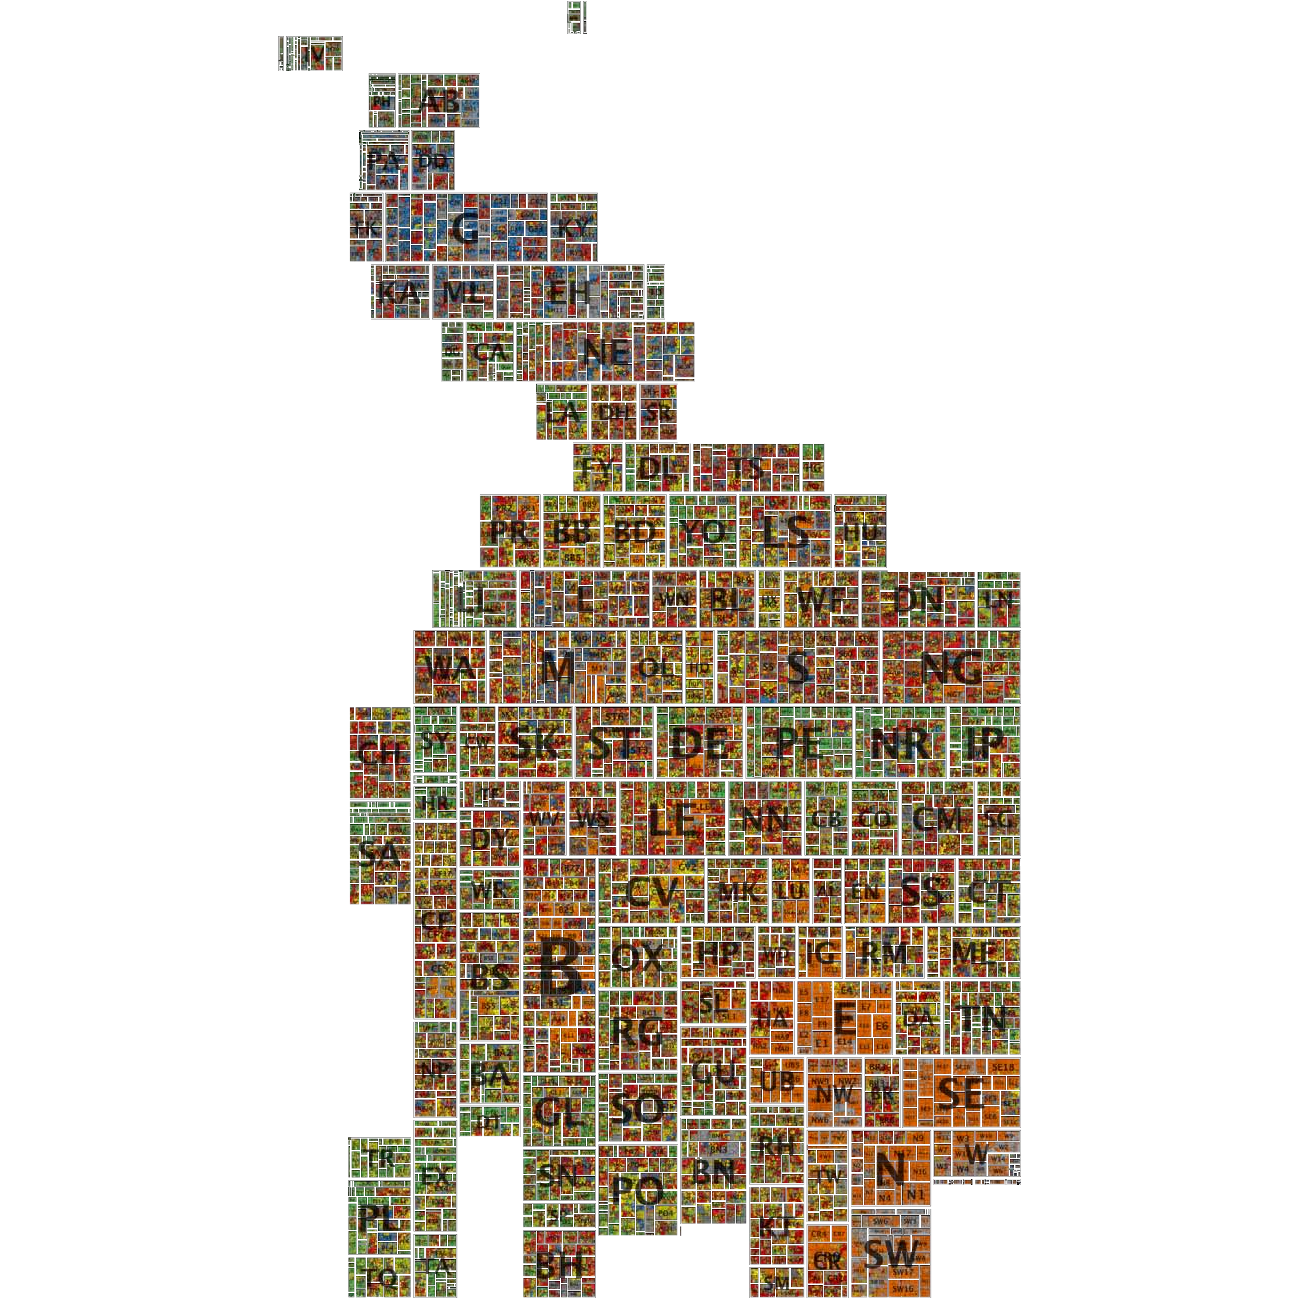
\includegraphics[width=\examplesdefaultwidth]{figures/cartogram.png}};
	\node[below=5pt of sot-5,text width=\examplesdefaultwidth,align=center] (sot-5-label) { Rectangular Hierarchical Cartogram };
	\node[above=5pt of sot-3] (Tc) { \Tc };
	\draw[thin,black,shorten >= 10pt] (Tc-|sot-1.west) -- (Tc);
	\draw[thin,black,shorten <= 10pt] (Tc) -- (Tc-|sot-5.east);
	\end{tikzpicture}
	\caption{Examples of treemaps from the category \emph{Containment Treemap}. Image courtesy from left to right: \cite{itoh2004-reactanglepacking}, \cite{scheibel2018-evocells}, \cite{wettel2007-cities}, \cite{wetzel2003-pebbles}, and \cite{slingsby2010-cartograms}.}
	\label{fig:TM1-examples}
\end{figure*}
\begin{figure*}[p]
	\centering
	\footnotesize
	\begin{tikzpicture}[every node/.style={inner sep=0,outer sep=0},node distance=0pt]
	\node[] (sot-1) {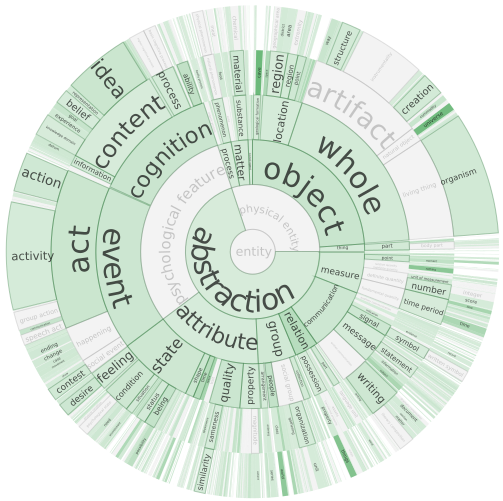
\includegraphics[width=\examplesdefaultwidth]{figures/sunburst.png}};
	\node[below=5pt of sot-1,text width=\examplesdefaultwidth,align=center] (sot-1-label) { Sunburst View };
	\node[right=10pt of sot-1] (sot-2) {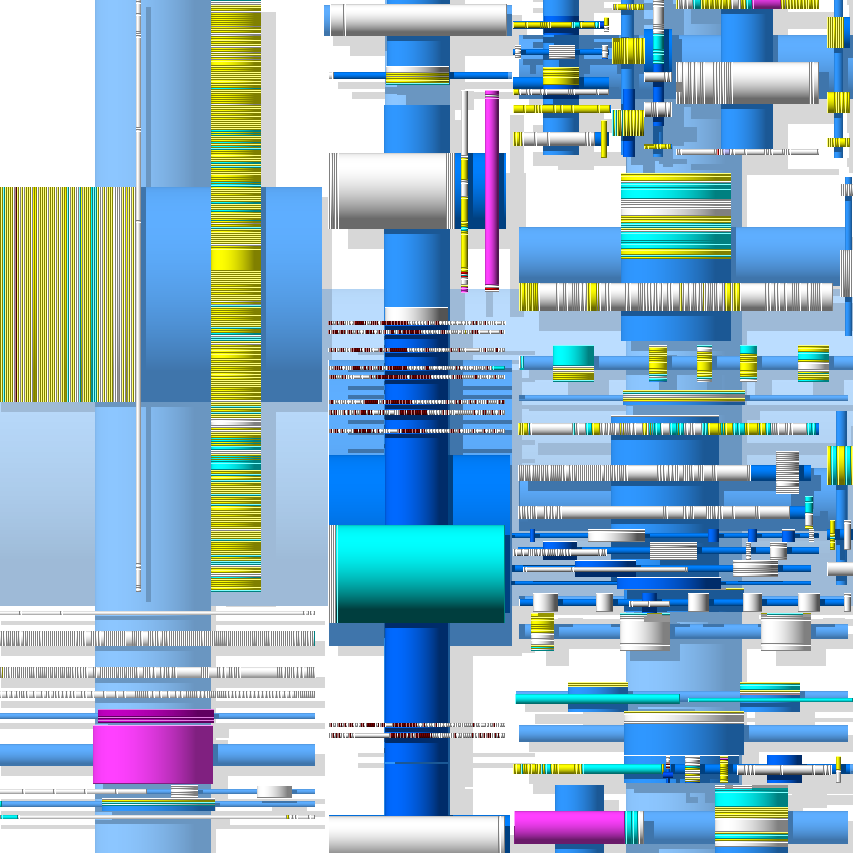
\includegraphics[width=\examplesdefaultwidth]{figures/beamtree-hr.png}};
	\node[below=5pt of sot-2,text width=\examplesdefaultwidth,align=center] (sot-2-label) { BeamTree };
	\node[right=10pt of sot-2] (sot-3) {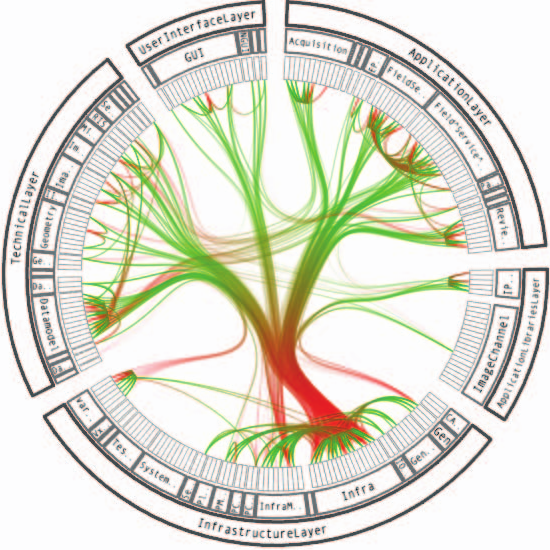
\includegraphics[width=\examplesdefaultwidth]{figures/bundleview.png}};
	\node[below=5pt of sot-3,text width=\examplesdefaultwidth,align=center] (sot-3-label) { Bundle View };
	\node[right=10pt of sot-3] (sot-4) {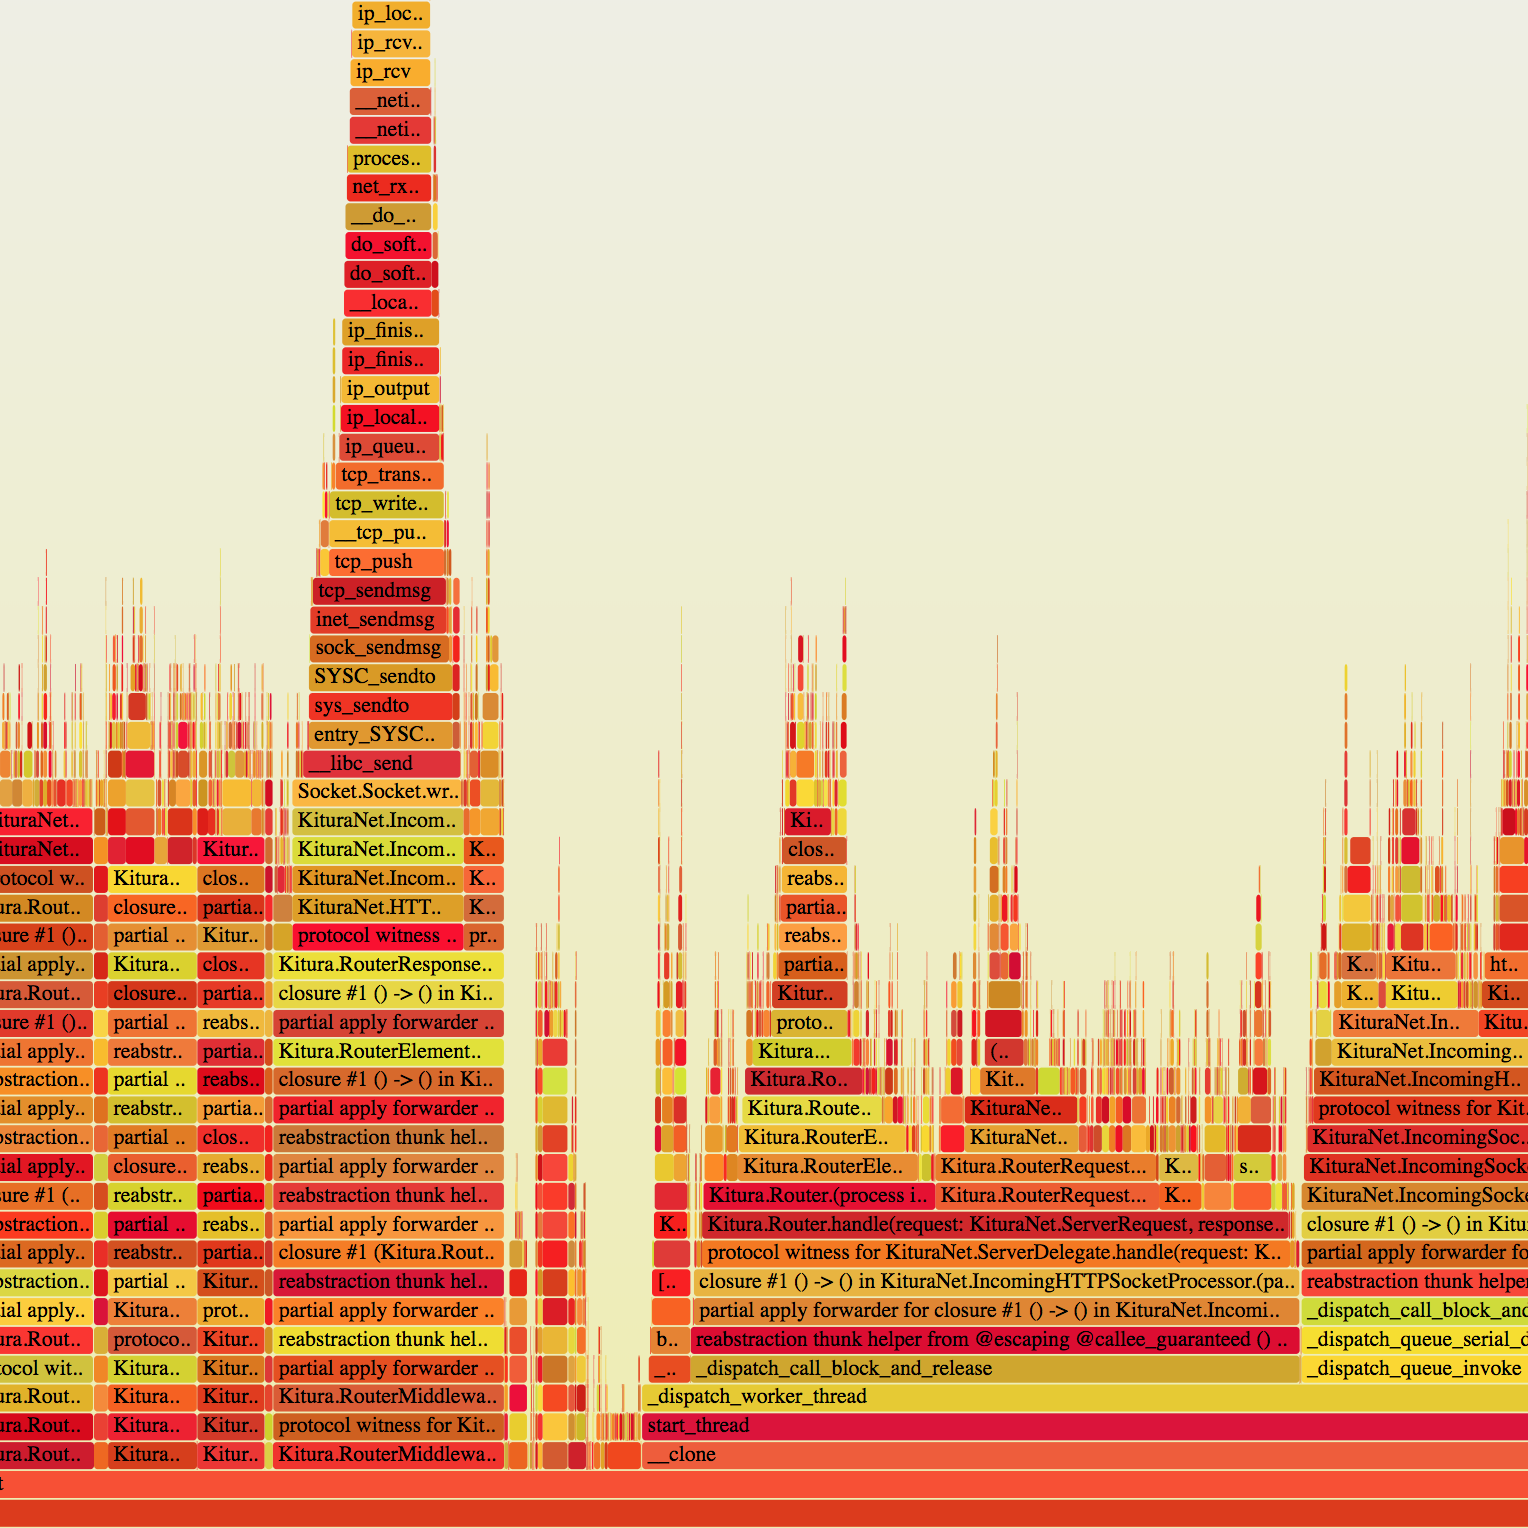
\includegraphics[width=\examplesdefaultwidth]{figures/flamegraph-hr.png}};
	\node[below=5pt of sot-4,text width=\examplesdefaultwidth,align=center] (sot-4-label) { Flame Graphs };
	\node[right=10pt of sot-4] (sot-5) {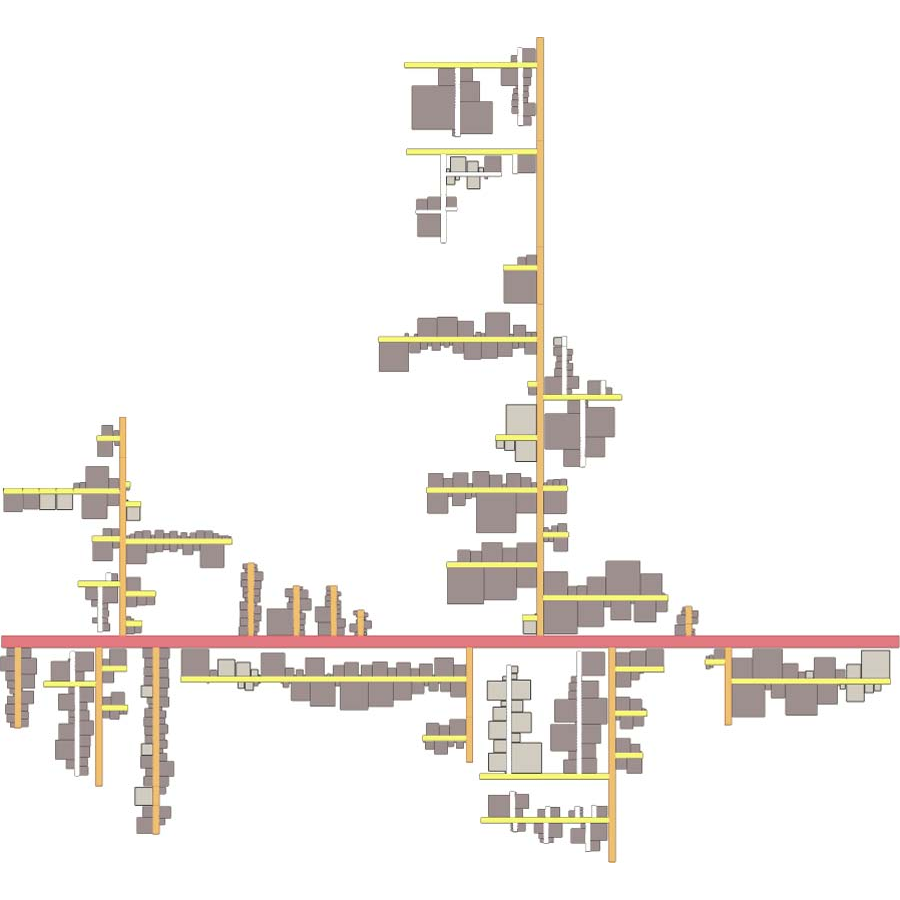
\includegraphics[width=\examplesdefaultwidth]{figures/evostreets.png}};
	\node[below=5pt of sot-5,text width=\examplesdefaultwidth,align=center] (sot-5-label) { Software Cities };
	\node[above=5pt of sot-3] (Tie) { \Tie };
	\draw[thin,black,shorten >= 10pt] (Tie-|sot-1.west) -- (Tie);
	\draw[thin,black,shorten <= 10pt] (Tie) -- (Tie-|sot-5.east);
	\end{tikzpicture}
	\caption{Examples of treemaps from the category \emph{Implicit Edge-Representation Treemap}. Image courtesy from left to right: \cite{stasko2000-structures}, \cite{vanHam2003-beamtrees}, \cite{holten2006-edgebundles}, \cite{gregg2016-flamegraphs}, and \cite{steinbruckner2013-evolution}.}
	\label{fig:TM2-examples}
\end{figure*}
\begin{figure*}[p]
	\centering
	\footnotesize
	\begin{tikzpicture}[every node/.style={inner sep=0,outer sep=0},node distance=0pt]
	\node[] (sot-1) {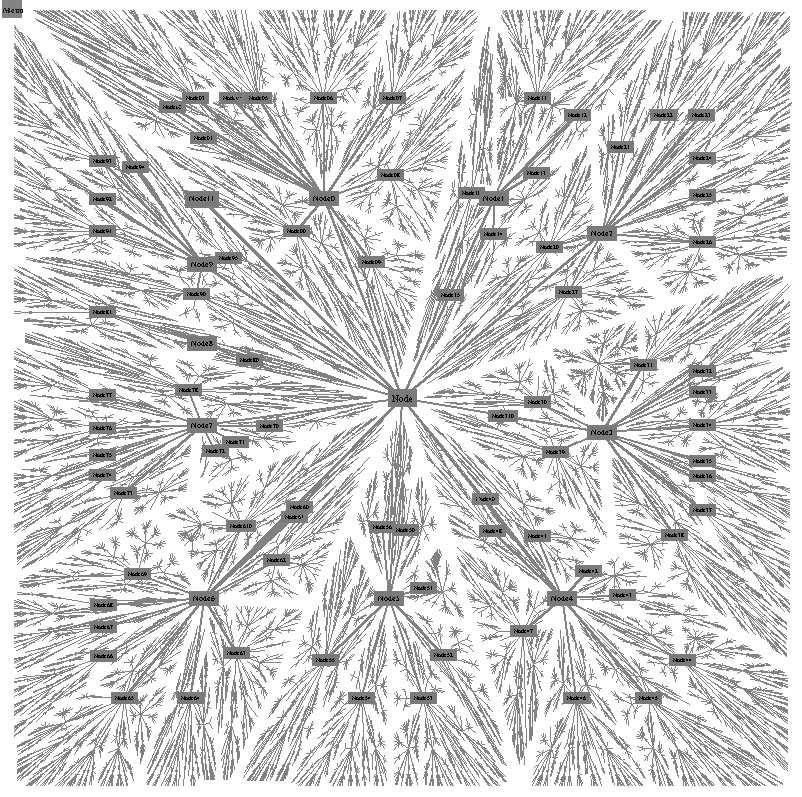
\includegraphics[width=\examplesdefaultwidth]{figures/spaceoptimizedtree.png}};
	\node[below=5pt of sot-1,text width=\examplesdefaultwidth,align=center] (sot-1-label) { Space-optimized Tree };
	\node[right=10pt of sot-1] (sot-2) {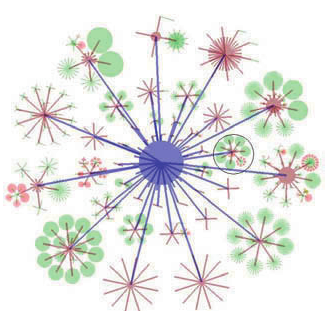
\includegraphics[width=\examplesdefaultwidth]{figures/rings.png}};
	\node[below=5pt of sot-2,text width=\examplesdefaultwidth,align=center] (sot-2-label) { RINGS };
	\node[right=10pt of sot-2] (sot-3) {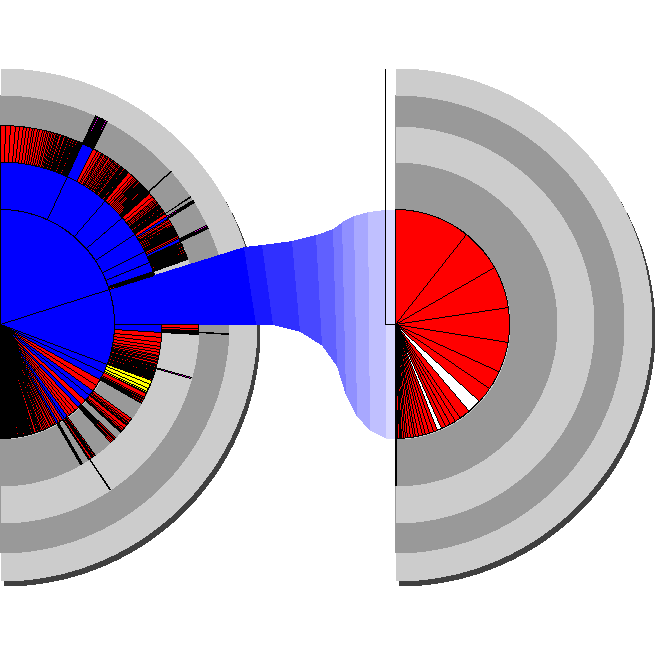
\includegraphics[width=\examplesdefaultwidth]{figures/informationslices.png}};
	\node[below=5pt of sot-3,text width=\examplesdefaultwidth,align=center] (sot-3-label) { Information Slices };
	\node[right=10pt of sot-3] (sot-4) {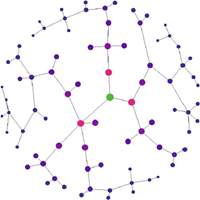
\includegraphics[width=\examplesdefaultwidth]{figures/circular-tree-drawing.png}};
	\node[below=5pt of sot-4,text width=\examplesdefaultwidth,align=center] (sot-4-label) { Tree Drawings };
	\node[right=10pt of sot-4] (sot-5) {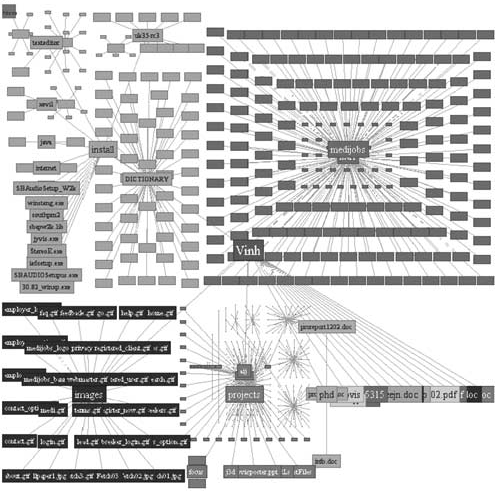
\includegraphics[width=\examplesdefaultwidth]{figures/enccon.png}};
	\node[below=5pt of sot-5,text width=\examplesdefaultwidth,align=center] (sot-4-label) { ENCCON };
	\node[above=5pt of sot-3] (Tmt) { \Tmt };
	\draw[thin,black,shorten >= 10pt] (Tmt-|sot-1.west) -- (Tmt);
	\draw[thin,black,shorten <= 10pt] (Tmt) -- (Tmt-|sot-5.east);
	\end{tikzpicture}
	\caption{Examples of treemaps from the category \emph{Mapped Tree}. Image courtesy from left to right: \cite{nguyen2002-sot}, \cite{teoh2002-rings}, \cite{andrews1998-slices}, \cite{toosi2014-circular}, and \cite{nguyen2005-enccon}.}
	\label{fig:TM3-examples}
\end{figure*}
\begin{figure*}[t]
	\centering
	\footnotesize
	\begin{tikzpicture}[every node/.style={inner sep=0,outer sep=0},node distance=0pt]
	\node[] (sot-1) {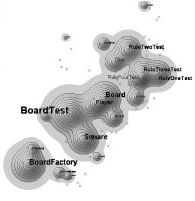
\includegraphics[width=\examplesdefaultwidth]{figures/thematicsoftwaremaps.png}};
	\node[below=5pt of sot-1,text width=\examplesdefaultwidth,align=center] (sot-1-label) { Thematic Software Maps };
	\node[right=10pt of sot-1] (sot-2) {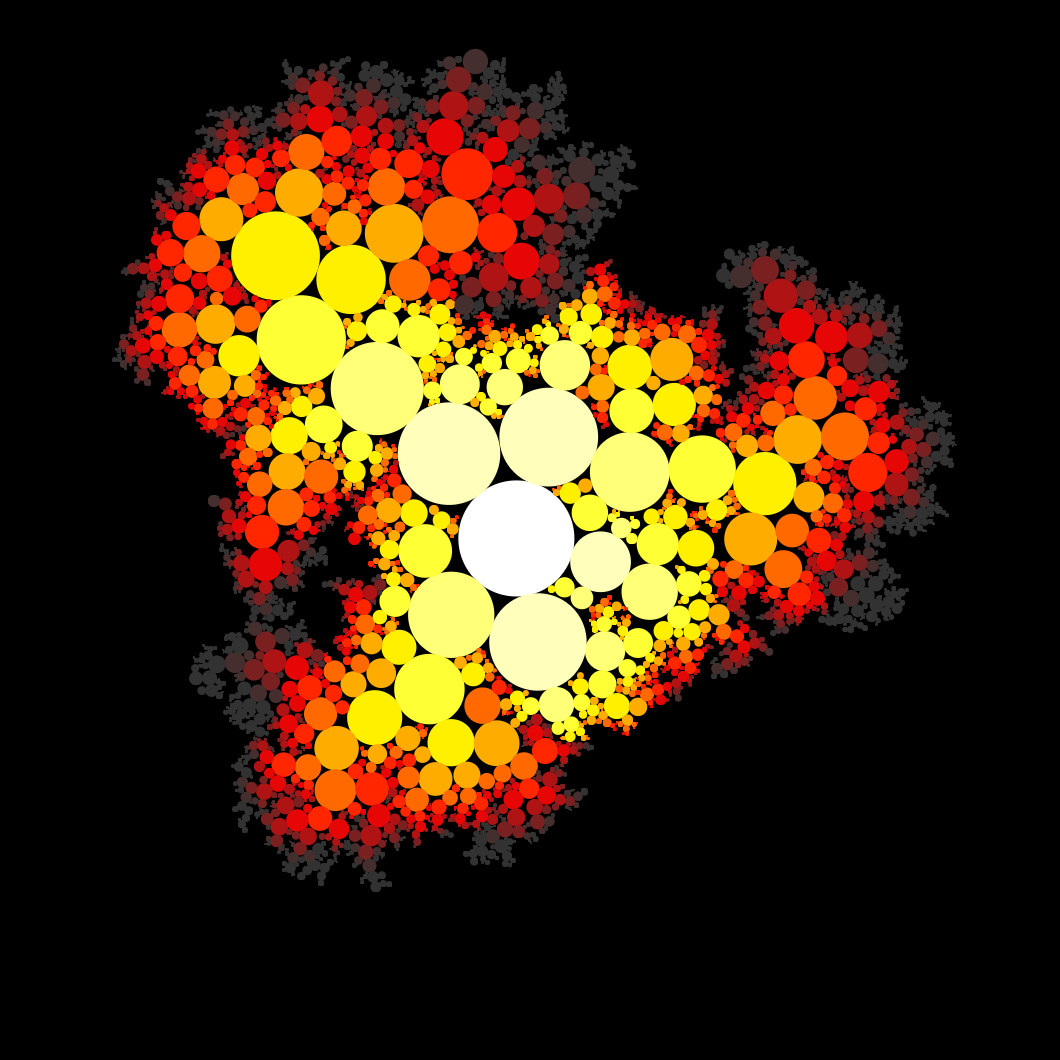
\includegraphics[width=\examplesdefaultwidth]{figures/bubblehierarchy.png}};
	\node[below=5pt of sot-2,text width=\examplesdefaultwidth,align=center] (sot-2-label) { Bubble Hierarchies };
	\node[right=10pt of sot-2] (sot-3) {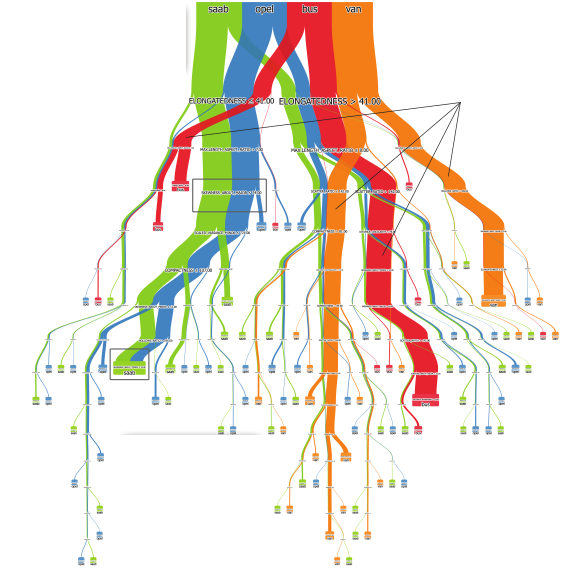
\includegraphics[width=\examplesdefaultwidth]{figures/baobabview.png}};
	\node[below=5pt of sot-3,text width=\examplesdefaultwidth,align=center] (sot-3-label) { BaobabView };
	\node[right=10pt of sot-3] (sot-4) {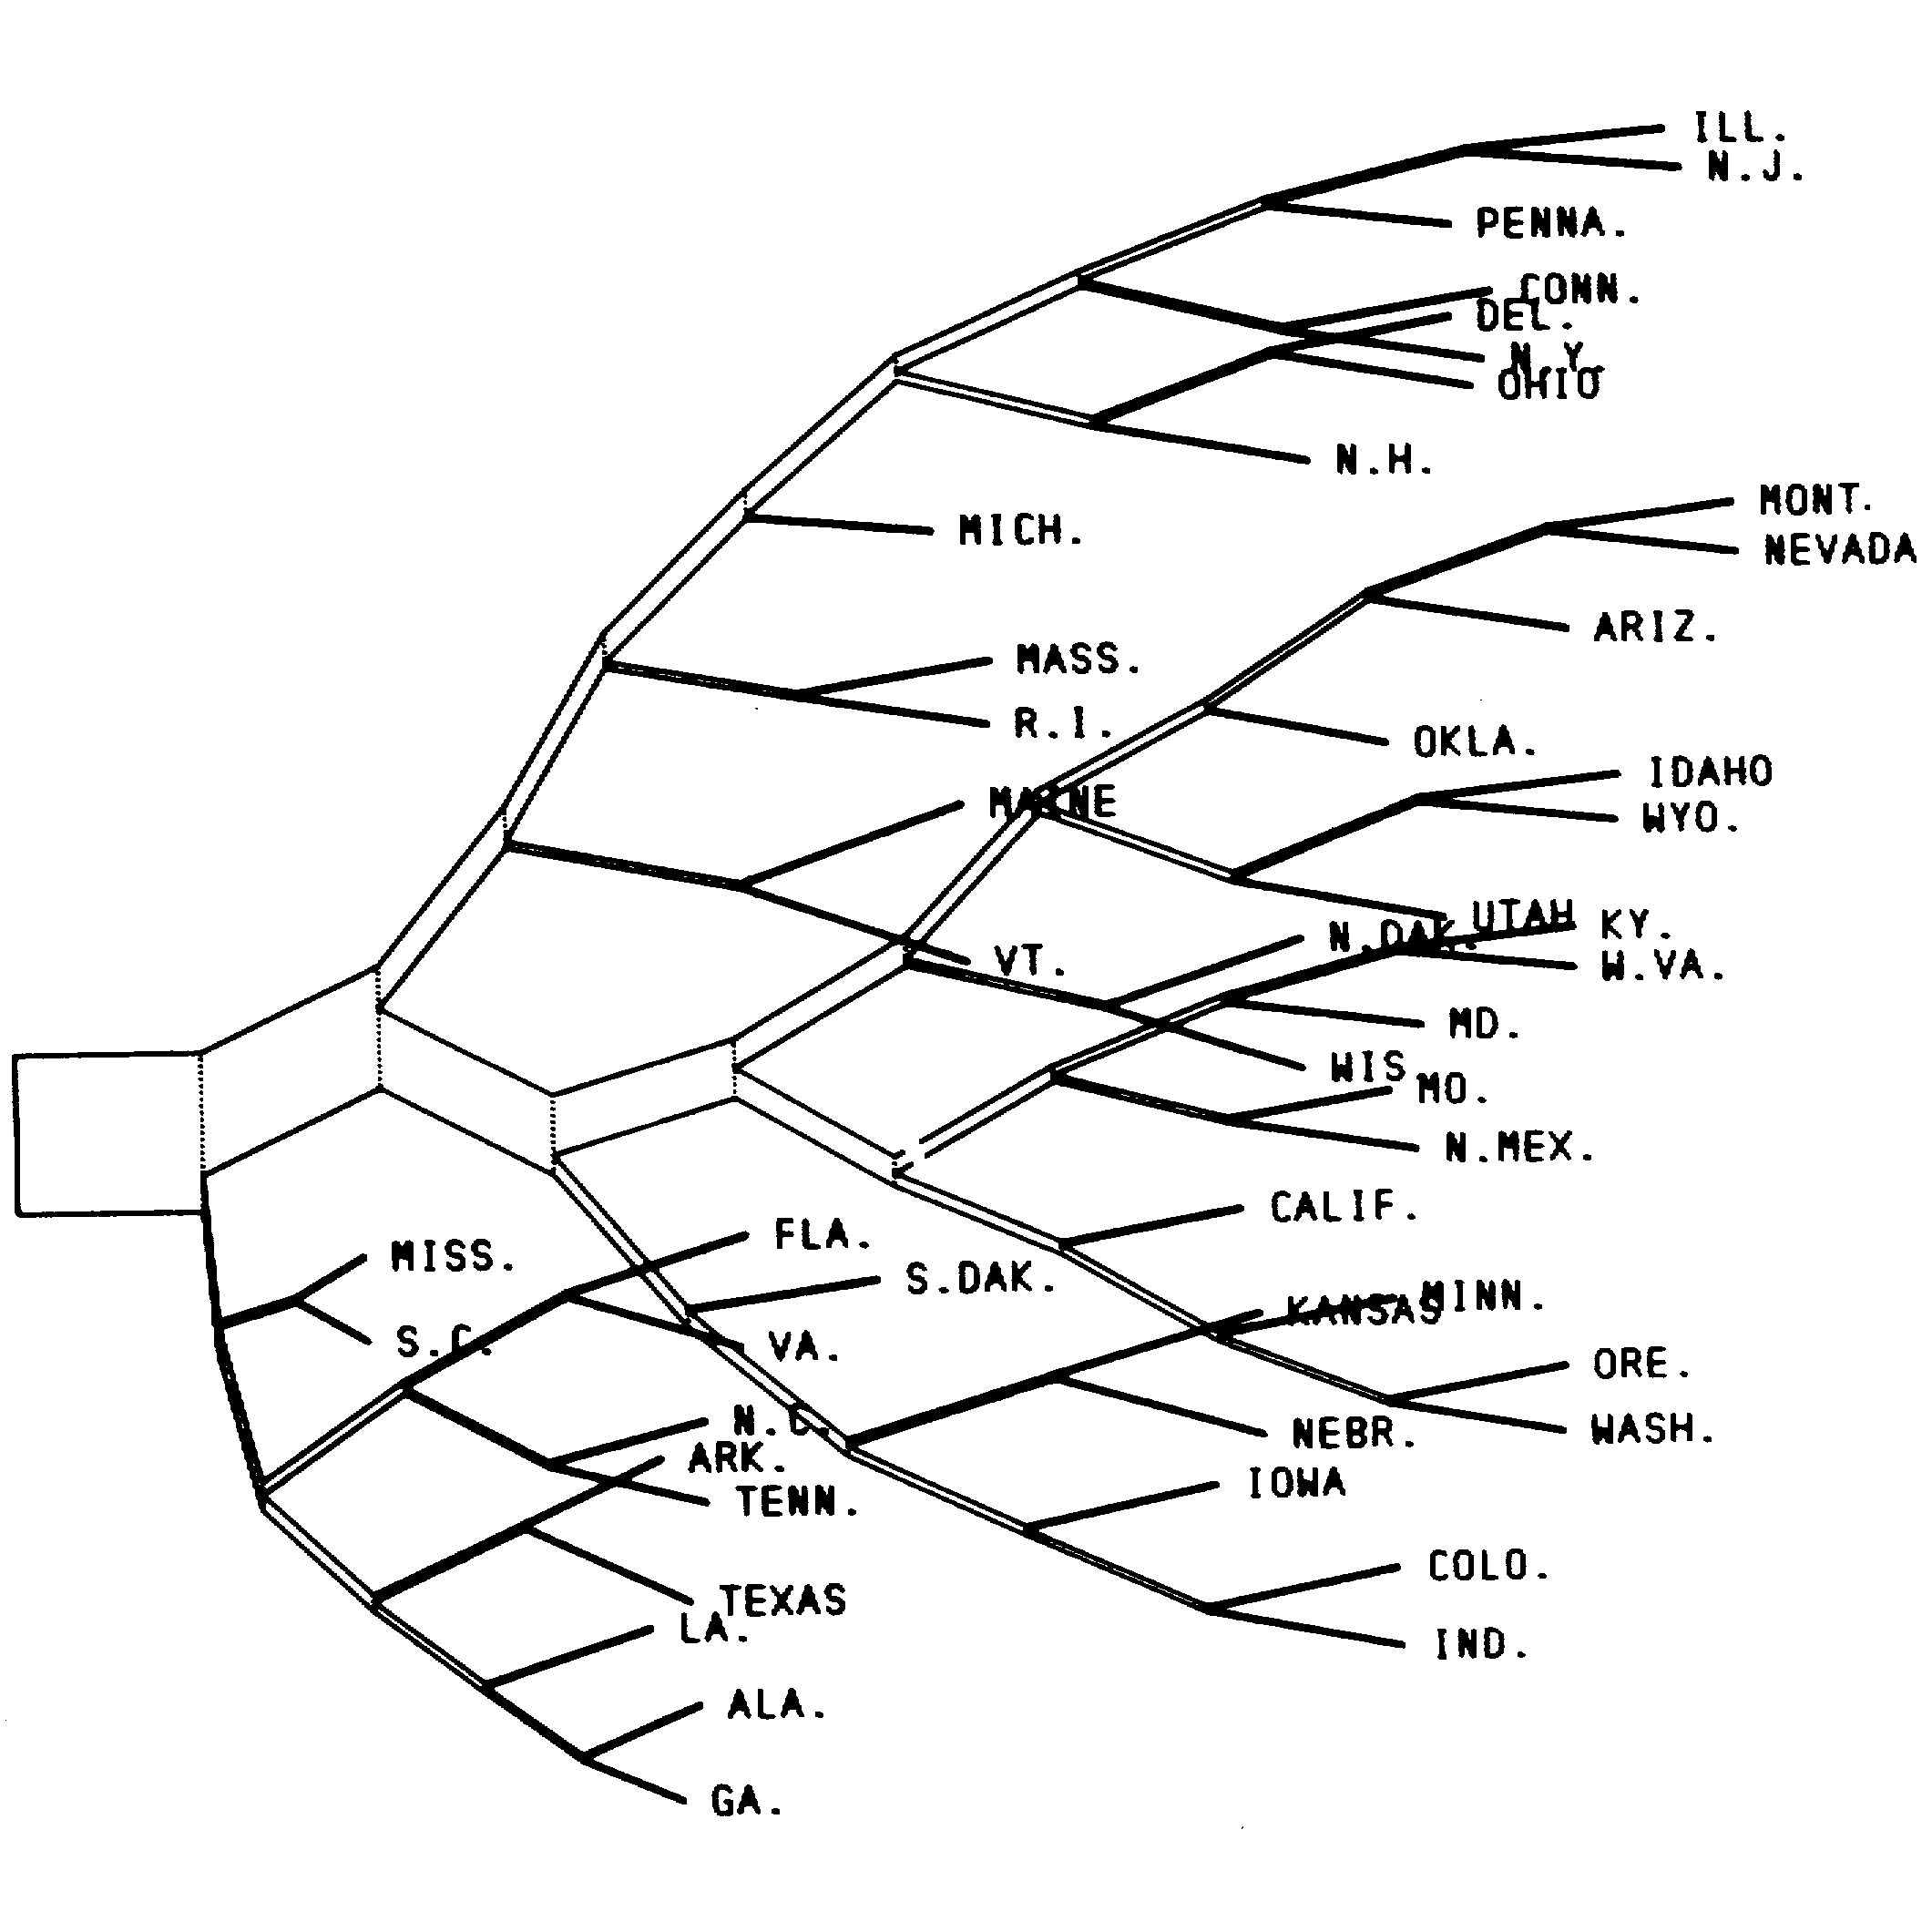
\includegraphics[width=\examplesdefaultwidth]{figures/tree.png}};
	\node[below=5pt of sot-4,text width=\examplesdefaultwidth,align=center] (sot-4-label) { Tree of Percentage };
	\node[right=10pt of sot-4] (sot-5) {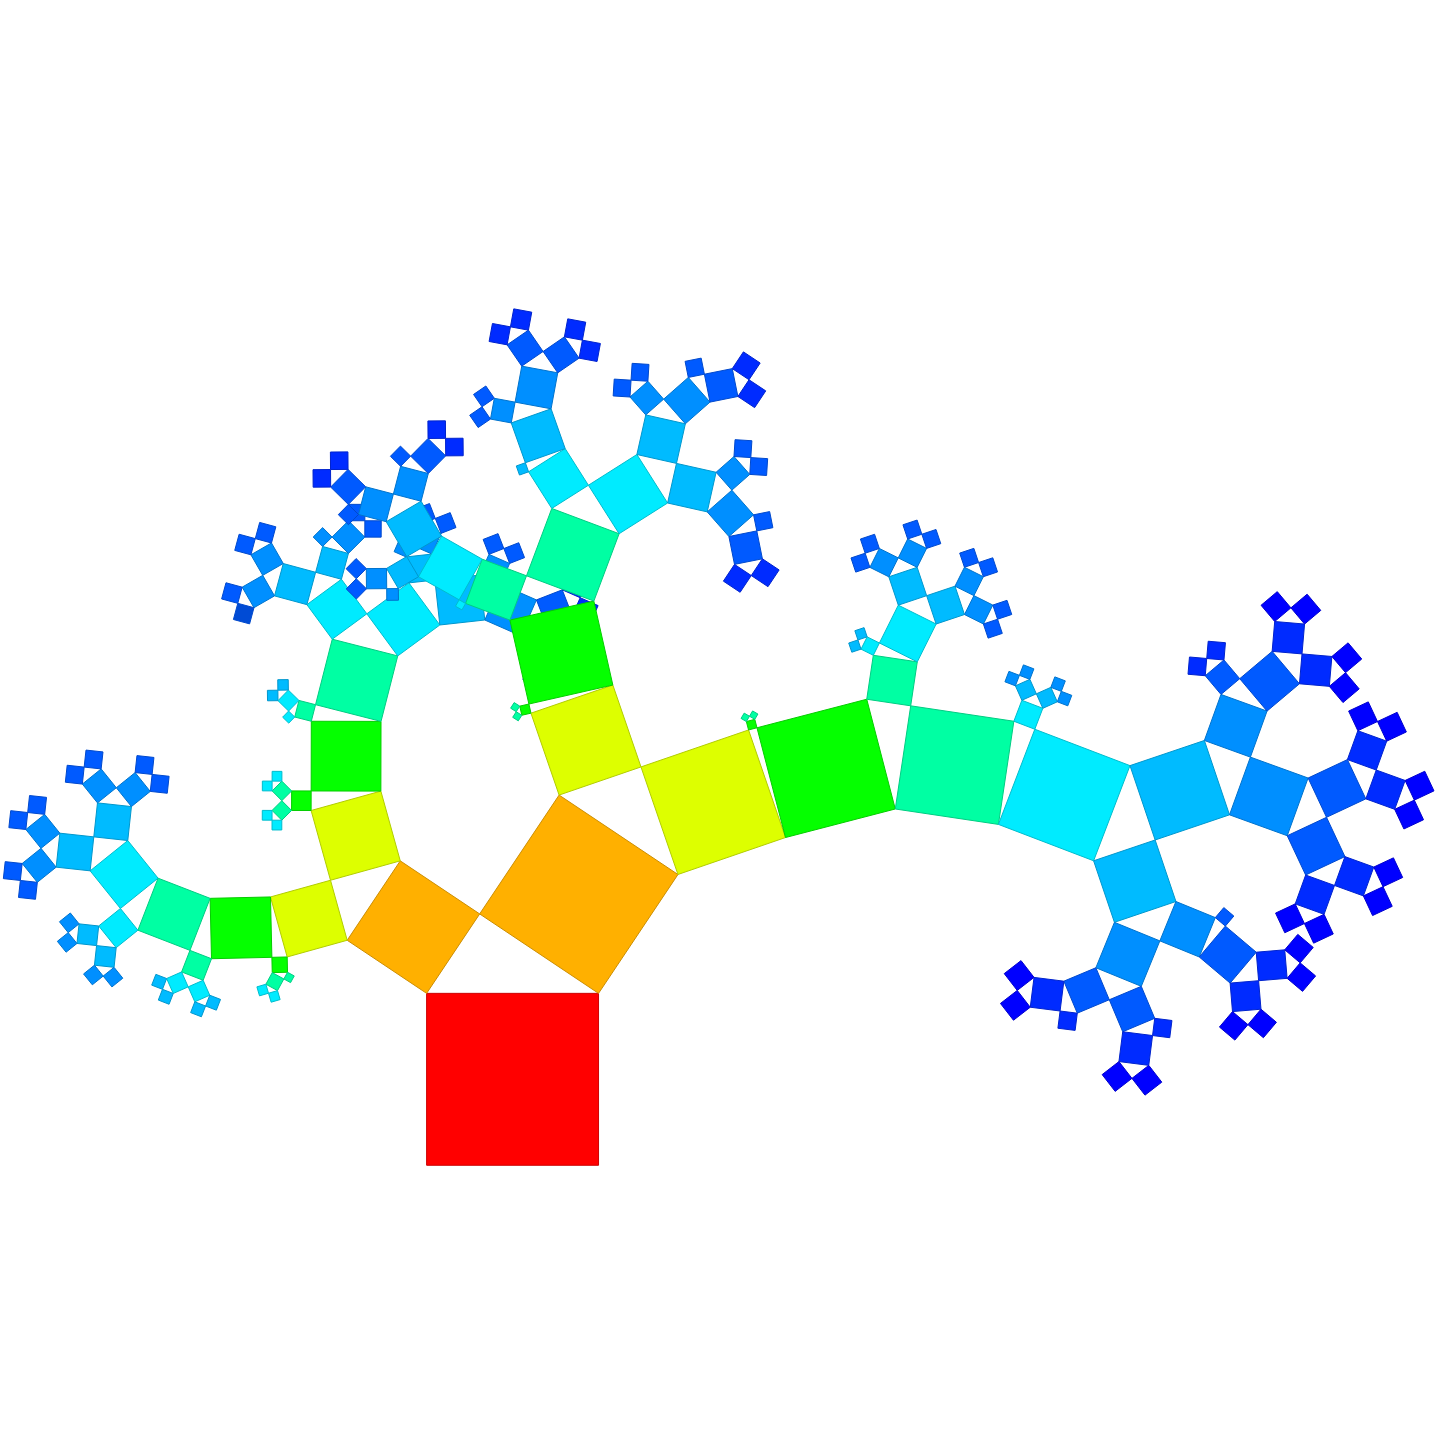
\includegraphics[width=\examplesdefaultwidth]{figures/pythagorastree.png}};
	\node[below=5pt of sot-5,text width=\examplesdefaultwidth,align=center] (sot-5-label) { Pythagoras Tree };
	\node[above=5pt of sot-3] (Th) { \Th };
	\draw[thin,black,shorten >= 10pt] (Th-|sot-1.west) -- (Th);
	\draw[thin,black,shorten <= 10pt] (Th) -- (Th-|sot-5.east);
	\end{tikzpicture}
	\caption{Examples of visualization techniques that does not relate to any proposed class and are therefore associated with \Th{}. Image courtesy from left to right: \cite{kuhn2010-thematic}, \cite{hlawatsch2014-bubblehierarchies}, \cite{andrews1998-slices}, \cite{elzen2011-baobabtrees}, and \cite{kleiner1981-trees}, and \cite{beck2014-pythagorastrees}.}
	\label{fig:TM4-examples}
\end{figure*}

\section{\uppercase{Discussion}}
\noindent
When we categorize techniques of hierarchy visualization we aim at the most specific category.
As an example, the appropriate category of a CodeCity visualization is a containment treemap \Tc{}.
Through the taxonomy's hyponymous nature, the more general categories \Tie{} and \Tmt{} are valid as well, and so is the category of general hierarchy visualization techniques \Th{} (\autoref{fig:TM4-examples}).
However, we want to argue for a more specific use of terms (\autoref{tab:association}).
\par
The proposed taxonomy is derived from visual features of the visualization techniques.
Common to all categories is the property of containment from their underlying layouts.
As alternatives to the focus on visual features, the categorization could be based on the initial use of a containment-based layout.
This would render all techniques that are classified as mapped trees \Tmt{} as treemap.
\par
The actual boundary between mapped trees \Tmt{} and general hierarchy visualization techniques \Th{} remains to be determined.
We argue that only with a systematic top-down or bottom-up approach that adheres to the containment metaphor during layouting, the resulting visualization technique can result in a treemap.
That is, hierarchy visualization techniques using other approaches may not ensure overlap-free sibling nodes for the underlying layouts, e.g., Pythagoras Trees~\cite{beck2014-pythagorastrees}.
For those techniques, we observe their categorization as mapped tree \Tmt{} as soon as they achieve overlap-free sibling nodes~\cite{munz2019-pythagorastrees}.
\par
Regarding the mixed use of treemap visualization with other approaches, this taxonomy is explicitly designed ignorant.
As a debatable example, the mixed-projection treemap could be categorized as either \Ts{} or \Tie{}~\cite{limberger2017-mixed}.
Another example is the adjacent usage of treemaps by means of small multiples.
It may not inherently render the whole visualization a treemap, although the composition could be labeled a space-filling treemap \Ts{}~\cite{scheibel2016-smallmultiples}.
A constrasting example thereto is the CodeSurveyor visualization that uses an overlap-free distribution of the uppermost level and, in fact, should be labeled a containment treemap \Tc{}~\cite{hawes2015-codesurveyor}.

\section{\uppercase{Conclusions}}
\label{sec:conclusions}
\noindent
This paper proposes a taxonomy for treemap visualization techniques, namely \emph{Space-filling Treemap} \Ts, \emph{Containment Treemap} \Tc, \emph{Implicit Edge Representation Tree} \Tie, and \emph{Mapped Tree} \Tmt.
This is feasible because all associated techniques adhere to the property of \emph{containment}, either in their visual representation or in their underlying layout.
Furthermore, the taxonomy should clarify the labeling of visualization techniques as treemaps and improve communication on their characteristics, visual metaphors, internally used algorithms, and interaction techniques.
\par
As future work, the classification of existing hierarchy visualization techniques by means of the proposed taxonomy should be continued.
We suggest to integrate the conceptual model of these different classes into hierarchy visualization systems and their APIs~\cite{scheibel2019-hiviser}.
Right now, we stimulate this discussion on a classification of treemaps and, probably, a broadening of the concept of treemaps and their role within the field of hierarchy visualization.

\section*{\uppercase{Acknowledgements}}
\noindent%
This work was partially funded by %
the German Federal Ministry for Economic Affairs and Energy (BMWi, ZIM) within the project \enquote{{TASAM}}.

\bibliographystyle{apalike}
{
\small
\bibliography{treemap-categories}
}

\end{document}
